% !TEX encoding = UTF-8 Unicode
% !TEX TS-program = pdflatex

\documentclass[
	corpo=12pt,
	twoside,
 	evenboxes,
	tipotesi=triennale,
    	stile=classica,
   	 greek,
]{toptesi}

\usepackage[utf8]{inputenc}
\usepackage[T1]{fontenc}
\usepackage[italian]{babel}
\usepackage{lmodern}
\usepackage{hyperref}
\usepackage{listings}
\usepackage{float}
\usepackage{booktabs}
\usepackage{xcolor}
\usepackage[style=alphabetic, labelnumber, defernumbers=true,  backend=biber]{biblatex}
\usepackage{guit}
\usepackage{filecontents}

\hypersetup{
	pdfpagemode={UseOutlines},
	bookmarksopen,
	pdfstartview={FitH},
	colorlinks,
	linkcolor={black},
	citecolor={black},
	urlcolor={black}
}

% Listing (Codice)
\lstset{frame=tb,
  language=Java,
  aboveskip=3mm,
  belowskip=3mm,
  showstringspaces=false,
  columns=flexible,
  basicstyle={\fontsize{10}{12}\ttfamily},
  numbers=left,
  numberstyle=\tiny\color{black},
  keywordstyle=\color{black}\bfseries,
  commentstyle=\color{darkgray},
  stringstyle=\color{red},
  breaklines=true,
  breakatwhitespace=true,
  tabsize=3
}

% Definizioni locali
\newtheorem{osservazione}{Osservazione}

% French spacing
\frenchspacing

% Interlinea
\linespread{1.25}

% Lipsum
\usepackage{lipsum}

\begin{filecontents*}{bibliography.bib}
@misc{pestneil,
author = {Neil Carter},
title = {PEST (Parameter Estimation by Sequential Testing)},
url = {psy.swansea.ac.uk/staff/carter/projects/PEST_explanation.htm},
year = {2017}
}

@misc{ambliopia,
author = {Humanitas},
title = {Ambliopia},
url = {www.humanitas.it/malattie/ambliopia-occhio-pigro},
year = {2017}
}

@misc{pestalex,
author = {Alex Pentlando},
title = {Maximum likelihood estimation: The best PEST},
publisher = {Perception \& Psychophysics},
number = {Volume 28-4},
year = {1980}
}

@misc{pest,
author = {M. M. Taylor and C. Douglas Creelman},
title = {PEST: Efficient Estimates on Probability Functions},
publisher = {Journal of the Acoustical Society of America},
number = {Volume 41-4},
year = {1967}
}
\end{filecontents*}

\begin{filecontents*}{sitography.bib}
@online{3d4amb,
title = {3D4AMB},
url = {3d4amb.unibg.it}
}

@online{se4med,
title = {SE4MED},
url = {se4med.unibg.it}
}

@online{androiddevelopers,
title = {Android Developers},
url = {developer.android.com}
}

@online{codecover,
title = {CodeCover},
url = {codecover.org}
}

@online{eclipse,
title = {Eclipse},
url = {eclipse.org}
}

@online{mysql,
title = {MySQL},
url = {mysql.com}
}

@online{json,
title = {JSON},
url = {json.org}
}

@online{jooq,
title = {JOOQ},
url = {jooq.org}
}

@online{github,
title = {GitHub},
url = {github.com}
}

@online{stacloverflow,
title = {Stack Overflow},
url = {stackoverflow.com}
}
\end{filecontents*}

\addbibresource{bibliography.bib}
\addbibresource{sitography.bib}

% Append keywords to identify different bibliography entries
\DeclareSourcemap{
  \maps[datatype=bibtex, overwrite]{
    \map{
      \perdatasource{bibliography.bib}
      \step[fieldset=KEYWORDS, fieldvalue=primary, append]
    }
    \map{
      \perdatasource{sitography.bib}
      \step[fieldset=KEYWORDS, fieldvalue=secondary, append]
    }
  }
}

\DeclareFieldFormat{labelnumberwidth}{\mkbibbrackets{#1}}
\renewbibmacro*{cite}{%
  \printtext[bibhyperref]{%
    \printfield{labelprefix}%
    \ifkeyword{secondary}
      {\printfield{labelnumber}}
      {\printfield{labelalpha}%
       \printfield{extraalpha}}}}


\defbibenvironment{bibliographyNUM}
  {\list
     {\printtext[labelnumberwidth]{%
        \printfield{prefixnumber}%
        \printfield{labelnumber}}}
     {\setlength{\labelwidth}{\labelnumberwidth}%
      \setlength{\leftmargin}{\labelwidth}%
      \setlength{\labelsep}{\biblabelsep}%
      \addtolength{\leftmargin}{\labelsep}%
      \setlength{\itemsep}{\bibitemsep}%
      \setlength{\parsep}{\bibparsep}}%
      \renewcommand*{\makelabel}[1]{\hss##1}}
  {\endlist}
  {\item}

\assignrefcontextkeyws[sorting=none]{secondary}

\begin{document}

% \pagenumbering{roman}

\pagenumbering{gobble} 

\begin{ThesisTitlePage}
	\nomeateneo{Università degli studi di Bergamo}
	\StrutturaDi{Scuola di }
	\struttura{Ingegneria}
	\NomeElaborato{Tesi di laurea triennale}
	\titolo{3DSAT}
	\sottotitolo{Progettazione e sviluppo di 3D Stereo Acuity Test con algoritmo PEST (Parameter Estimation by Sequential Testing)}     
	\corsodistudi{Ingegneria Informatica\\Classe N. L-08 - Ingegneria dell’informazione (D.M. 270/04)}
	\candidato{Samuele FERRI [1045975]}
	\secondocandidato{Simone SUDATI [1045936]}
	\relatore{prof.~Angelo GARGANTINI}
	\secondorelatore{prof.ssa~Silvia BONFANTI}
	\sedutadilaurea{ANNO~ACCADEMICO 2018-2019}
	\logosede{images/unibg.png}
\end{ThesisTitlePage}

% Citazione
\iffalse % Inizio commento
\vspace*{\stretch{1}}
\begin{flushright}
\noindent
Citazione

\textit{Autore}
\end{flushright}
\vspace*{\stretch{6}}
\cleardoublepage
\fi % Fine commento

% Ringraziamenti
% \ringraziamenti

% Sommario
% \sommario

% Pagina vuota
\paginavuota 

\indici

\mainmatter

\pagenumbering{arabic}

% Parte
%\part{Prima Parte}

% Lipsum
%\lipsum[1-2]

%%%%% INTRODUZIONE GENERALE %%%%%
\chapter{Introduzione generale}
\label{chap:introduzionegenerale}

\section{Ambliopia}
\label{sec:ambliopia}
Il termine \textbf{ambliopia} deriva dal punto di vista etimologico dalla composizione in lingua greca di \textgreek{ὤψ} (vista) e \textgreek{ἀμβλύς} (pigra, debole). L'oftalmologia, che è la branca della medicina dell'apparato visivo, definisce l'ambliopia come l'alterazione della visione dello spazio; la motivazione è da ricercarsi in un'alterata trasmissione del segnale nervoso tra occhio e cervello per cui quest'ultimo privilegia un occhio a causa della ridotta acuità visiva dell'altro. Secondo statistiche dell'Humanitas Research Hospital \cite{ambliopia} essa è una condizione che interessa il 4\% della popolazione mondiale e per le conoscenze attuali può essere trattata con successo solo se riconosciuta entro i primi 5-6 anni di vita. Data la piccola età, raramente i segnali/sintomi sono riferiti dal paziente e per questo motivo si raccomanda la prevenzione anche in assenza di sintomi attraverso visite oculistiche e screening fin dai primi anni di vita del bambino.

In caso di ambliopia contratta bisogna passare al più presto al trattamento in collaborazione con gli ortottisti. Per curarla vi sono diversi trattamenti ma tutti fondati sullo stesso principio: quello di far "sforzare" maggiormente il cosiddetto occhio pigro. Per raggiungere questo scopo tra le varie tecniche annoveriamo l'occlusione diretta con bande adesive che può avvenire o direttamente sull'occhio o con filtri semitrasparenti posti sugli occhiali come in figura \ref{fig:occhio_pigro_ambliopia}.

\newpage

\begin{figure}[H]
\centering
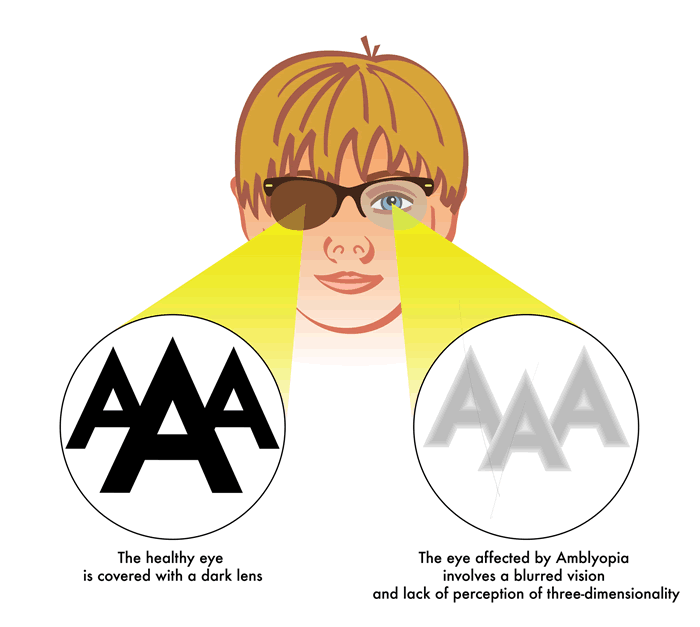
\includegraphics[width=0.70\columnwidth]{images/occhio_pigro_ambliopia.png}
\caption{Occlusione tramite filtri semitrasparenti (patching)}
\label{fig:occhio_pigro_ambliopia}
\end{figure}

Ulteriori tecniche riguardano la penalizzazione ottica con l'uso di supporti fisici. Un esempio sono gli occhiali con filtri di Bangerter, dove le lenti hanno gradi differenti di opacizzazione per l’inibizione dell’occhio sano e la stimolazione di quello ambliope.

Oltre alle tecniche fisiche esiste anche la penalizzazione farmacologica, ovvero la somministrazione di collirio a base di atropina
nell’occhio dominante. Questa sostanza dilata la pupilla rendendo così più difficoltosa la vista dall’occhio sano e stimolando conseguentemente l’occhio pigro ad attivarsi.

\newpage

\section{Stereoacuità}
\label{sec:stereoacuità}
La \textbf{stereoacuità visiva} anche detta percezione della profondità, è la più piccola differenza di profondità che può essere percepita tramite la visione binoculare tra due oggetti visibili.
Essa è una delle sottocategorie della cosiddetta "acuità di allineamento o localizzazione": l'acutezza visiva dovuta al minimo spostamento spaziale percepibile tra due figure.

La misura dell'acutezza stereoscopica ha come unità di misura i secondi d'arco (arcsec). Il suo multiplo, il minuto d'arco, indica la dimensione di un oggetto in angoli. Questa espressione della dimensione di un oggetto è utile in quanto la sua dimensione percepita cambia a seconda della distanza dell'osservatore dall'oggetto stesso. Un minuto d'arco sono 60 secondi d'arco e un grado sono 60 minuti d'arco. Quindi un grado è composto da 3600 secondi d'arco.

\[ 1'=60",\ 1^\circ =60' \Rightarrow 1^\circ=3600'' \]

\vfill

L'acutezza stereoscopica è la disparità minima oltre la quale non si produce alcun effetto stereoscopico. Più è piccolo l'angolo $\alpha$ e maggiore sarà l'acuità visiva secondo la legge \textit{tan}($\alpha$)\textit{=h/d} in cui $\alpha$ è in funzione della distanza della mira e dell'altezza. Valori pari a circa 15-30 secondi d’arco, ossia $0.004^\circ-0.008^\circ$, sono ritenuti eccellenti.

\begin{figure}[H]
\centering
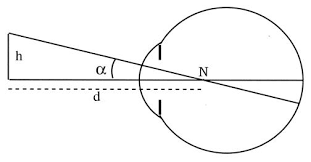
\includegraphics[width=0.55\columnwidth]{images/misurazione_stereoacuita.png}
\caption{Angolo $\alpha$ dell'acuità visiva}
\label{fig:misurazione_stereoacuita}
\end{figure}

Storicamente si sono delineate diverse tipologie di test che permettono di misurare la stereoacuità; il primo test fisico per la misurazione della stereo acuità è stato svolto da Howard-Dolman nel 1919.

\vfill

\newpage 

Il test, mostrato in figura \ref{fig:howard_dolman}, è così strutturato:
\begin{itemize}
\item Di fronte all'osservatore viene posto un piolo nero (A) ad una distanza $z$.
\item Un altro piolo nero (B) viene posto poco più avanti al primo, ad una distanza $dz$ che viene maneggiata finché B non viene percepito come il più vicino possibile a A.
\item A questo punto la distanza $dz$ viene convertita dall'unità di misura di lunghezza utilizzata all'unità di misura angolare di disparità binoculare (la differenza del paralasse binoculare) tramite la formula: 
\begin{equation}
d\gamma = cadz/z^2
\end{equation}
dove $c$ è una costante (3437.75, cioè 1 radiante in arcminuti), $a$ è la distanza interoculare dell'osservatore (la distanza tra occhio sinistro e occhio destro), $dz$ è la distanza minima della stereoacuità rilevata e $z$ la distanza tra gli occhi e il primo piolo A di riferimento.
\end{itemize}

\begin{figure}[H]
\centering
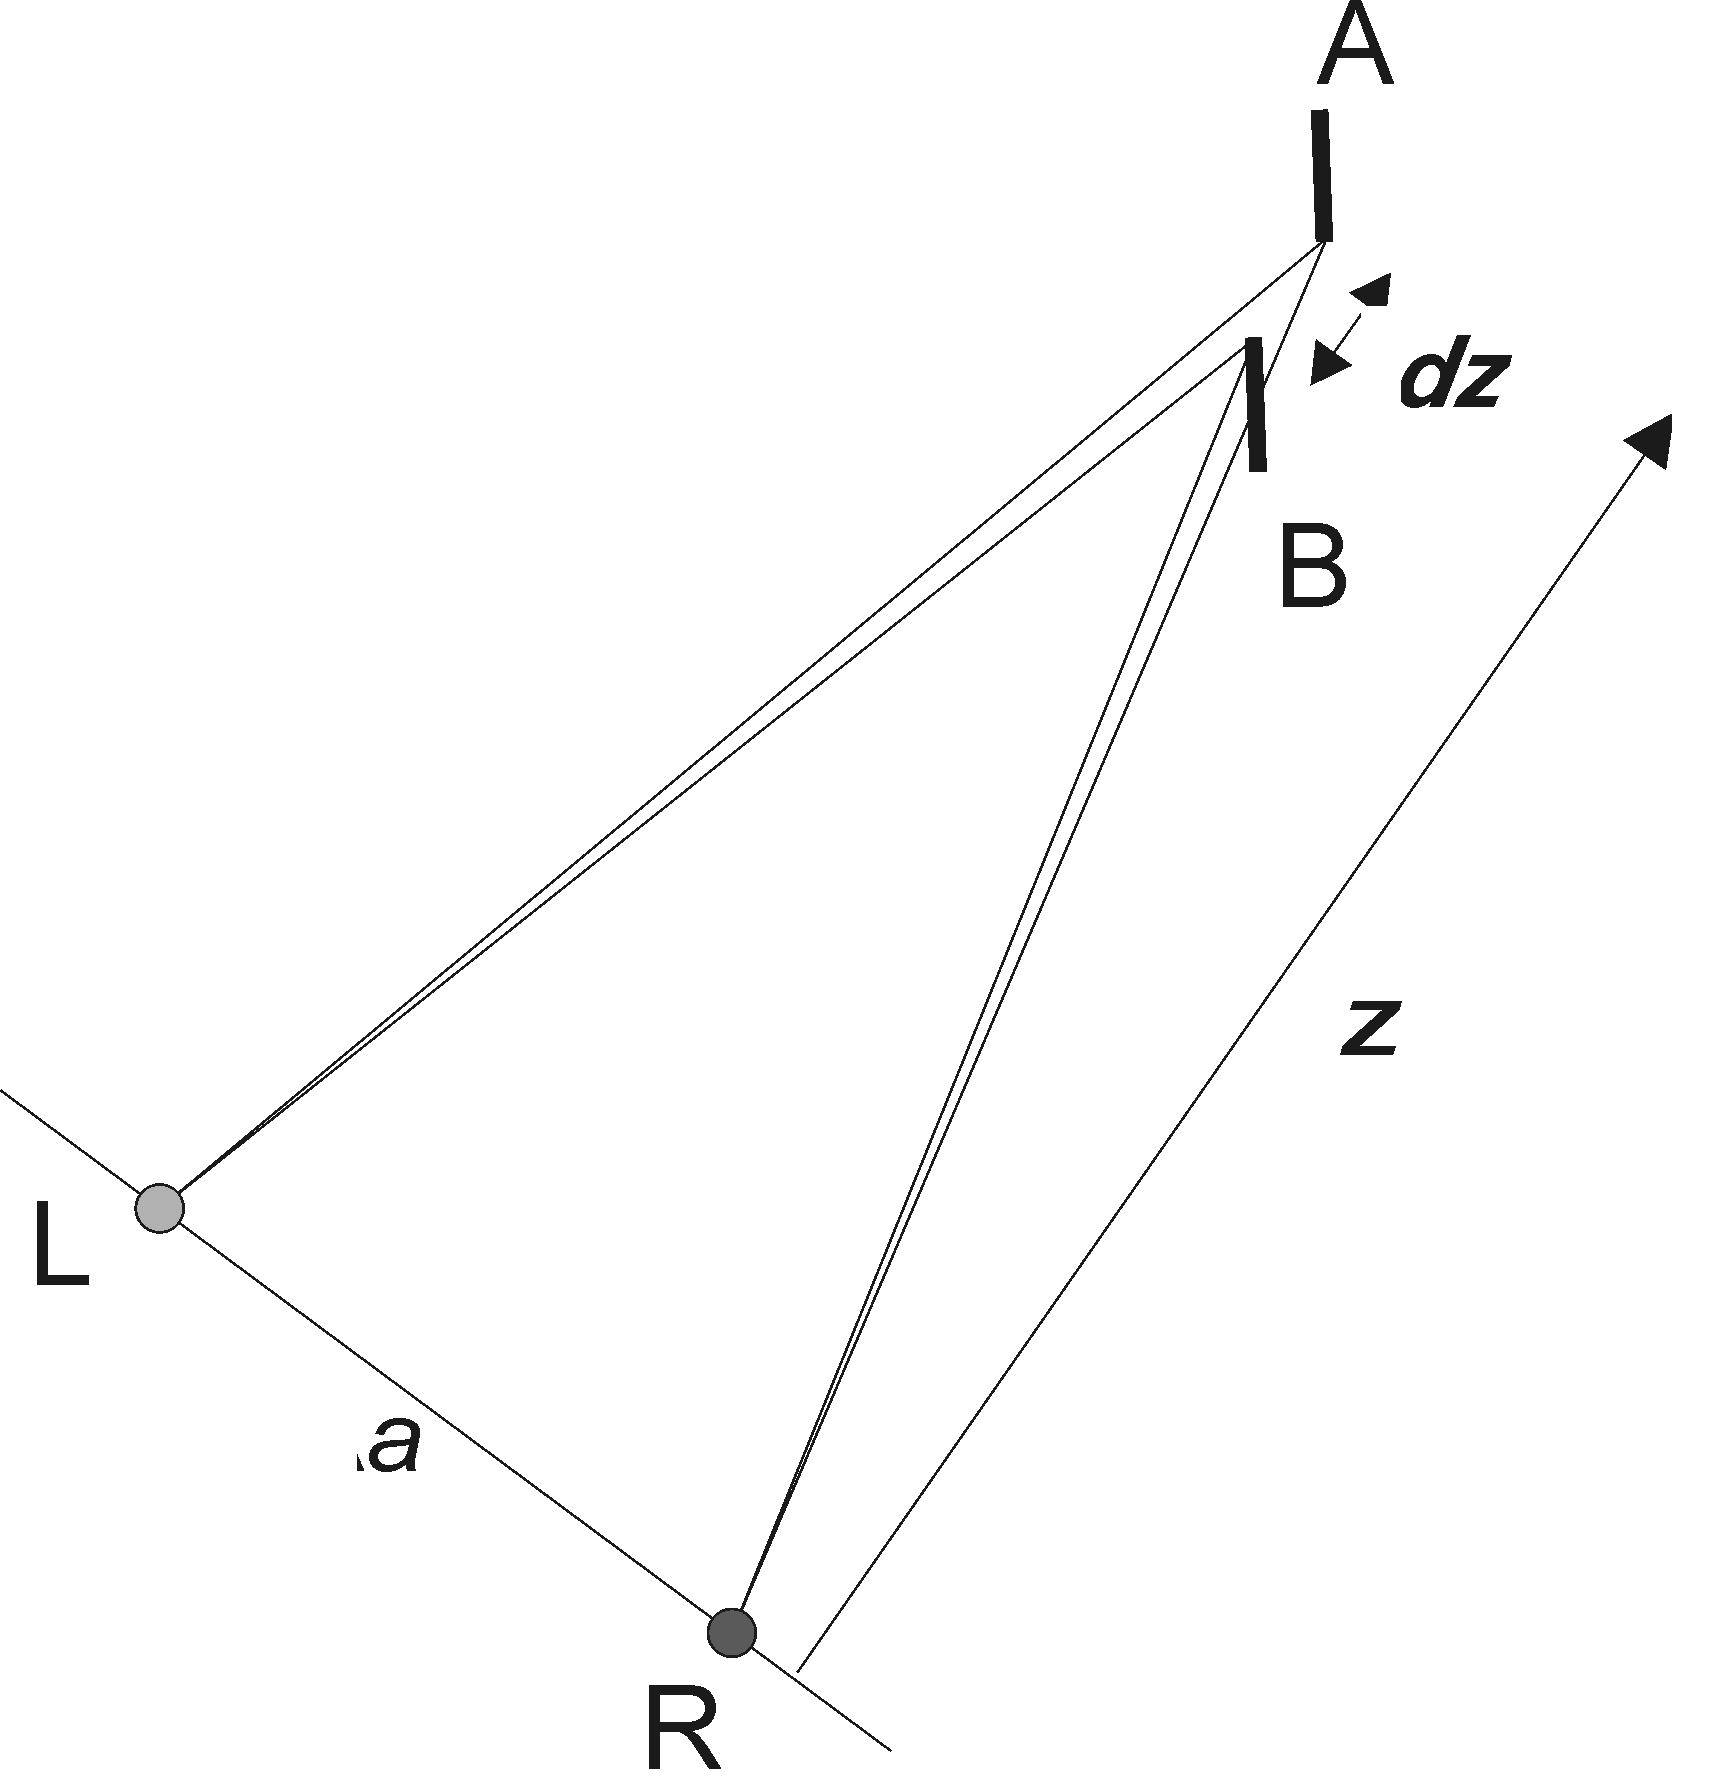
\includegraphics[width=0.40\columnwidth]{images/howard_dolman.png}
\caption{Rappresentazione grafica del test di Howard-Dolman}
\label{fig:howard_dolman}
\end{figure}

\newpage

\section{Anaglifi}
\label{sec:anaglifi}
Ora che abbiamo analizzato il funzionamento del test di stereoacuità in maniera fisica sorge una grossa problematica: per poter svolgere lo stesso test su schermi di dispositivi elettronici (cellullari nel nostro caso), che sono bidimensionali e virtuali, è necessaria un'astrazione per ottenere la tridimensionalità richiesta. Questa illusione la si ottiene con l'artificio degli anaglifi.

Un \textbf{anaglifo} è un'immagine stereoscopica che permette di avere un'illusione di realtà tridimensionale tramite l'uso di appositi occhiali dotati di due filtri di colore complementare tra loro (solitamente rosso, un colore additivo, e ciano, un colore sottrattivo). La visione binoculare permette all'uomo la visione su tre dimensioni. Questi occhiali usando i filtri permettono all'occhio di vedere solo parzialmente l'immagine completa, nascondendo la parte che viene schermata dalla lente.

\begin{figure}[H]
\centering
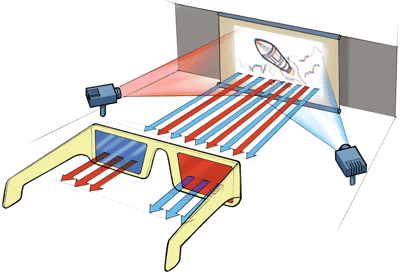
\includegraphics[width=0.55\columnwidth]{images/anaglifi.png}
\caption{Anaglifi}
\label{fig:anaglifi}
\end{figure}

L'idea alla base per ottenere lo stesso effetto tridimensionale è di avere due immagini del medesimo soggetto riprese alla stessa distanza ma scostate lateralmente con uno scarto pari alla distanza binoculare.

\newpage

\section{Il progetto 3D4AMB}
\label{sec:ilprogetto3d4amb}

\begin{figure}[H]
\centering

\includegraphics[width=0.50\columnwidth]{images/3d4amb.png}
\caption{Logo}
\label{fig:3d4amb}
\end{figure}
Il progetto \textbf{3D4AMB}\footnote{3D for the Diagnosis and Treatment of Amblyopia} \cite{3d4amb} è nato con l’obiettivo di sviluppare un sistema basato sul 3D per la diagnosi e il trattamento dell’ambliopia nei bambini piccoli. Utilizzando la tecnologia 3D è possibile mostrare immagini diverse all’occhio sano e a quello pigro, permettendo così di diagnosticare l’ambliopia in maniera più semplice e trattarla attraverso giochi interattivi e attività di intrattenimento.
I punti di forza principali del progetto 3D4AMB sono:

\begin{itemize}
\item \textbf{Basso costo}: i prodotti devono avere costi relativamente bassi, accessibili alle famiglie.
I componenti sono infatti acquistabili presso negozi e supermercati aperti ai privati cittadini.
\item \textbf{Ad uso domestico.} I sistemi sviluppati devono
poter essere installati ed utilizzati anche a casa. Questo eliminerebbe una parte
dei tragitti casa-clinica ed i tempi legati ad essi. In opportune condizioni, le 
terapie definite dai medici potranno quindi coprire periodi prolungati di erogazione
ed evitare quindi la necessità di contatti frequenti tra medico e paziente.

Per quanto riguarda i software di diagnosi, una loro versione opportunamente semplificata
potrebbe aiutare le scuole e il personale scolastico ad effettuare una prima, basilare
ed effettivamente precoce diagnosi nei casi più semplici, in modo da avvisare i genitori
che potranno accompagnare il figlio ad una prima visita oculistica.
\item \textbf{Facilmente estensibili.} I diversi software sviluppati dovranno essere
facilmente riutilizzabili ed estensibili con nuove funzionalità.
\end{itemize}

Il contesto in cui è inserito questo progetto è \textbf{SE4MED}\footnote{Software Engineering for Medical Devices} \cite{se4med}, un laboratorio dove si sviluppa software per dispositivi medici usando diverse tecnologie. In esso sono poste un insieme di iniziative e progetti sulla diagnosi e trattamento dell'ambliopia.

\section{Il nostro apporto}
\label{sec:ilnostroapporto}
All'interno di questo progetto, ci siamo concentrati sullo sviluppo e la miglioria di un'applicazione di supporto ai dottori per effettuare test sull'ambliopia ai bambini all'interno di scuole o incontri solo con l'ausilio di un cellulare e di occhialini anaglifici (rossi/blu). Nel caso in cui si rilevassero disparità visive elevate si potrà approfondire l'analisi con ulteriori strumenti e in caso affermativo iniziare un trattamento per la malattia.\\

Tecnicamente il nostro contributo può essere suddiviso su più fronti:
\begin{itemize}
\item Sviluppo di un'applicazione Android, base del nostro progetto arricchita di tutte le funzioni per permettere il test e i salvataggi dei risultati.
\item Aggiunta di ulteriori servizi in una servlet condivisa tra vari progetti di 3D4AMB per estendere le funzionalità dell'applicazione e il dialogo di quest'ultima con un database centrale presente sul server di SE4MED.
\item Implementazione di un nuovo algoritmo per la successione di immagini e il calcolo della disparità chiamato PEST\footnote{Parameter Estimation by Sequential Testing}. Esso è inserito all'interno di una libreria Java usata dalla nostra applicazione ma disponibile anche per altri progetti futuri. La principale finalità di questo nuovo algoritmo è di raggiungere, con un basso numero di prove da sottoporre in un test, il valore finale della disparità visiva del paziente. Oltre all'implementazione ci siamo anche occupati del testing di questo algoritmo per verificarne il corretto funzionamento.

Nei prossimi capitoli tratteremo di questi tre punti.
\end{itemize}

\vfill

%%%%% APPLICAZIONE %%%%%
\chapter{Applicazione}
\label{chap:applicazione}

\section{Introduzione all'applicazione}
\label{sec:introduzioneallapplicazione}
L'applicazione è la base principale del progetto, è composta da varie attività che si occupano di fornire funzioni e interfaccia all'utente. Nel nostro caso un dottore, il quale potrà gestire i propri pazienti, eseguire i test e salvare i risultati. L'applicazione è stata sviluppata in Java usando l'ambiente di sviluppo Android Studio \cite{androiddevelopers}, basandosi sulle API 23 in modo da rendere possibile l'esecuzione dell'applicazione su un maggior numero di dispositivi, compresi i meno recenti.\\

\begin{table}[]
\centering
\begin{tabular}{lllll}
\toprule
\textbf{Package} &  com.unibg.app3dsat (API 23)\\
\textbf{Tools} & Android Studio\\
\bottomrule
\end{tabular}
\caption{Dettagli applicazione \label{t:1}}
\end{table}

L'applicazione si interfaccia con una servlet (capitolo \ref{chap:servlet}) scritta in Java, la quale fornisce una serie di servizi consentendo di leggere e modificare un database centrale; proprio per questo motivo è necessaria una connessione a internet attiva per poter usare l'applicazione. 
L'applicazione si serve inoltre di una libreria (capitolo \ref{chap:libreria}) che abbiamo modificato introducendo un nuovo algoritmo chiamato PEST per il calcolo della disparità durante il test.

Nei prossimi paragrafi verranno analizzate le attività che compongono l'applicazione; infine verranno presentati alcuni dettagli tecnici e tecniche usate.

\newpage

\section{Main activities}
\label{sec:mainactivities}

\subsection{Login}
\label{subsec:login}
\begin{figure}[H]
\centering
\fbox{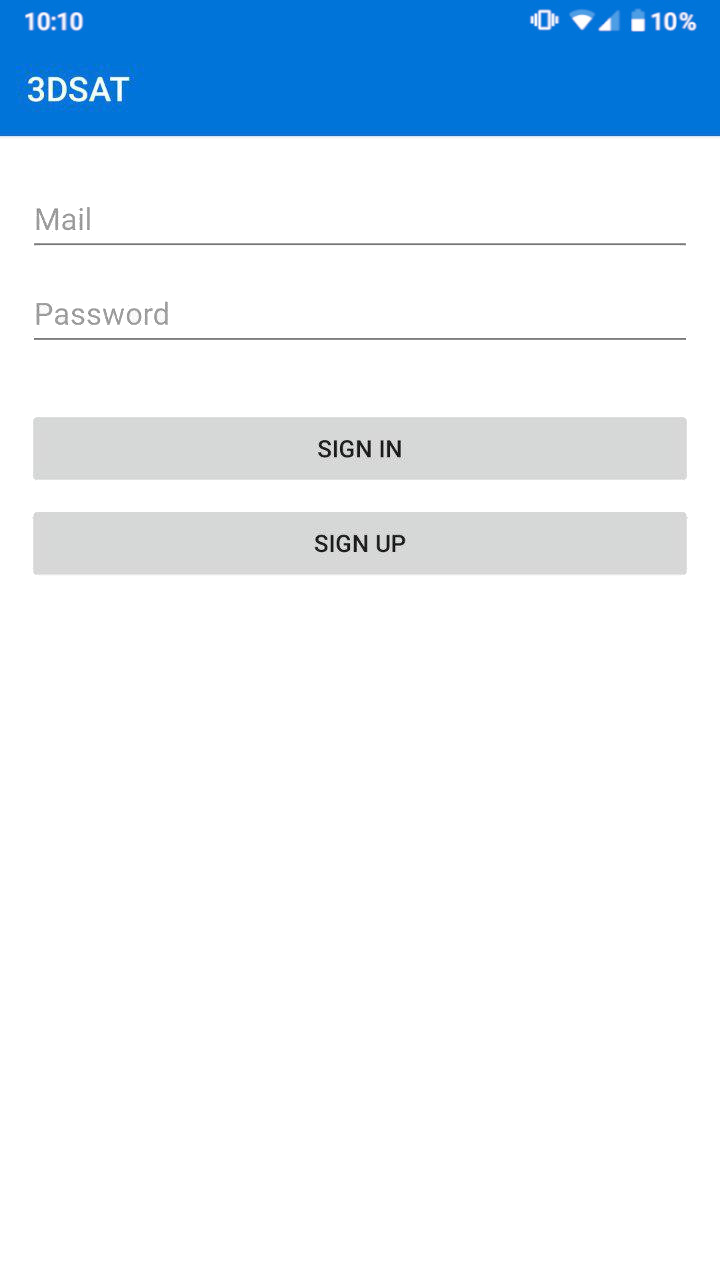
\includegraphics[width=0.35\columnwidth]{images/app_login.png}}
\caption{LoginActivity.java}
\label{fig:app_login}
\end{figure}
All'apertura dell'applicazione verrà presentato il form per il login del dottore. Le credenziali d'accesso possono essere ottenute dal dottore registrandosi su \textit{se4med.unibg.it/home}, sito raggiungibile facilmente cliccando il pulsante \textit{sign up}.
In caso di digitazione errata della password o errori di rete verrà visualizzato un messaggio di errore nell'interfaccia.

\vfill

\subsection{Main Doctor}
\label{subsec:maindoctor}
\begin{figure}[H]
\centering
\fbox{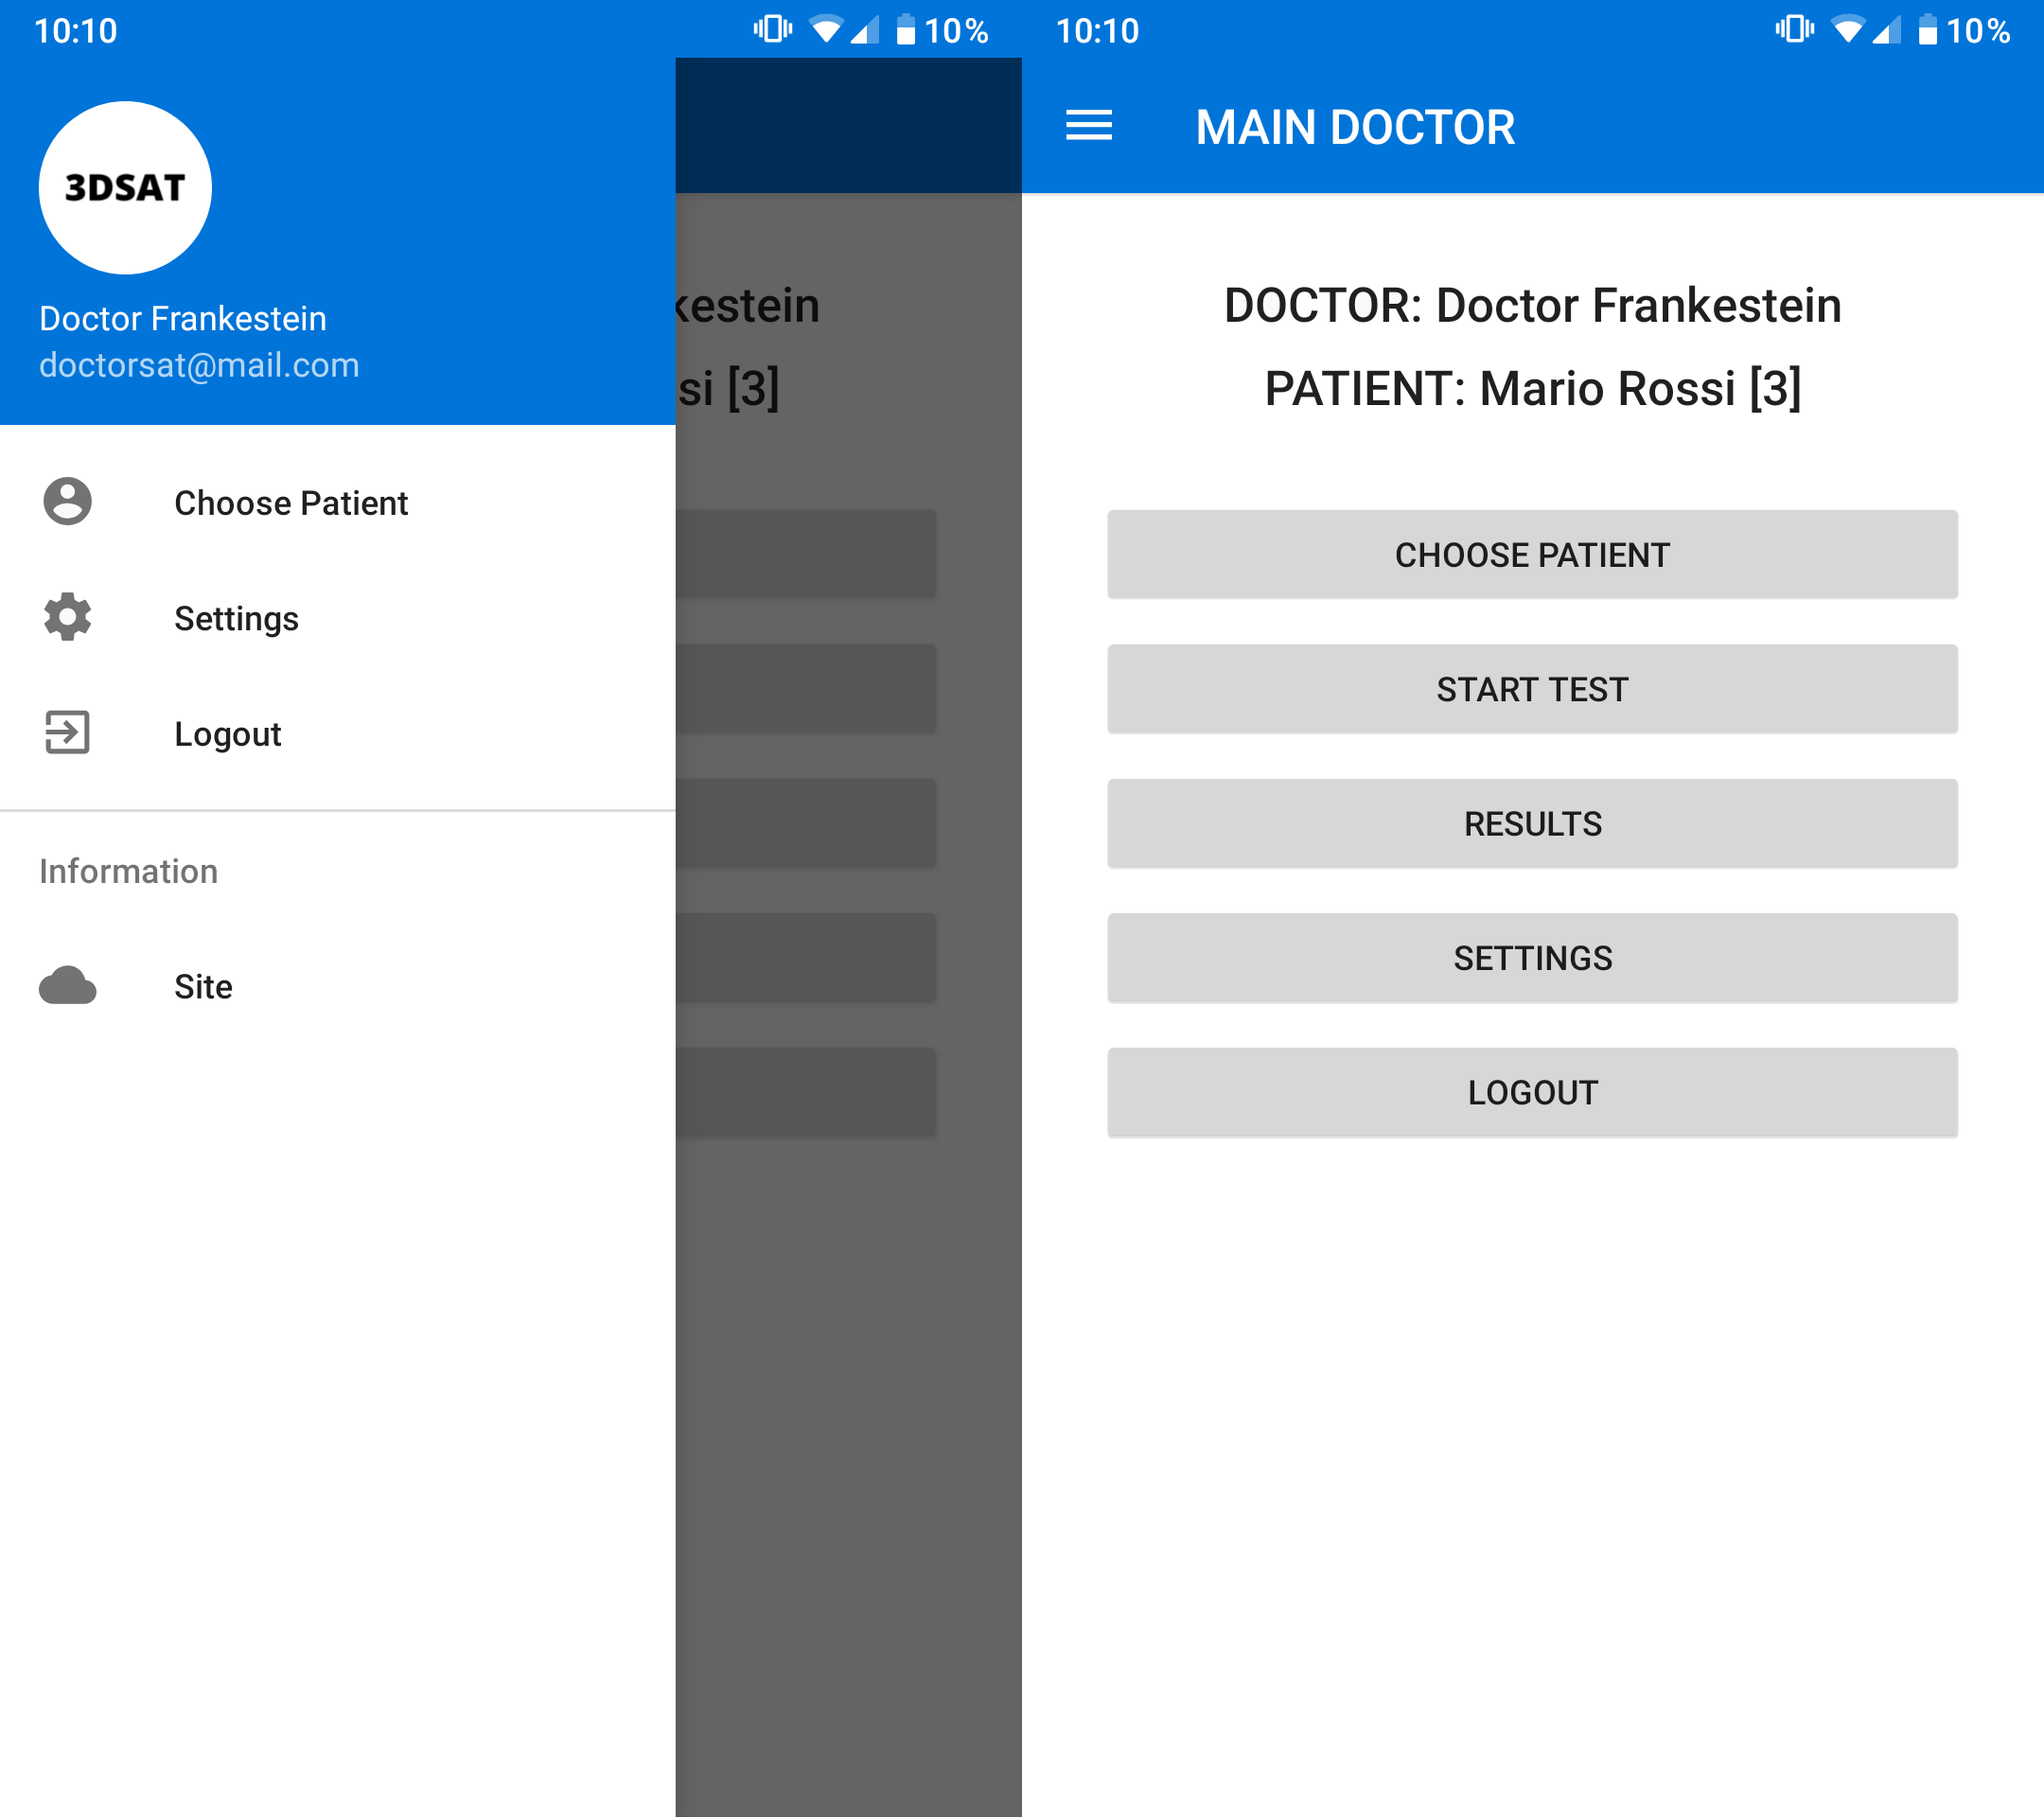
\includegraphics[width=0.70\columnwidth]{images/app_main_doctor_nav.png}}
\caption{MainDoctor.java}
\label{fig:app_main_doctor_nav}
\end{figure}
Dopo aver effettuato l'accesso correttamente, verrà presentato al dottore il menu principale compreso di navbar che riporta i dati del dottore. Sempre nella navbar è presente un collegamento alla versione web tramite un link al sito \textit{se4med.unibg.it/home}. Nell'intestazione troviamo anche il nome del paziente attualmente selezionato con il relativo ID; al primo accesso nell'applicazione non verrà visualizzato nulla, questo perché non è stato ancora selezionato/creato nessun paziente. È necessario quindi andare a selezionare/creare il paziente nell'apposita attività. 

Le sezioni per iniziare il test e per visualizzare i risultati sono accessibili soltanto se un paziente è stato correttamente selezionato.
Sarà inoltre possibile modificare le impostazioni dell'applicazione nell'apposita attività oppure effettuare il logout dal menu o dalla navbar e tornare al login form.
\vfill

\subsection{Main Patient}
\label{subsec:main patient}
\begin{figure}[H]
\centering
\fbox{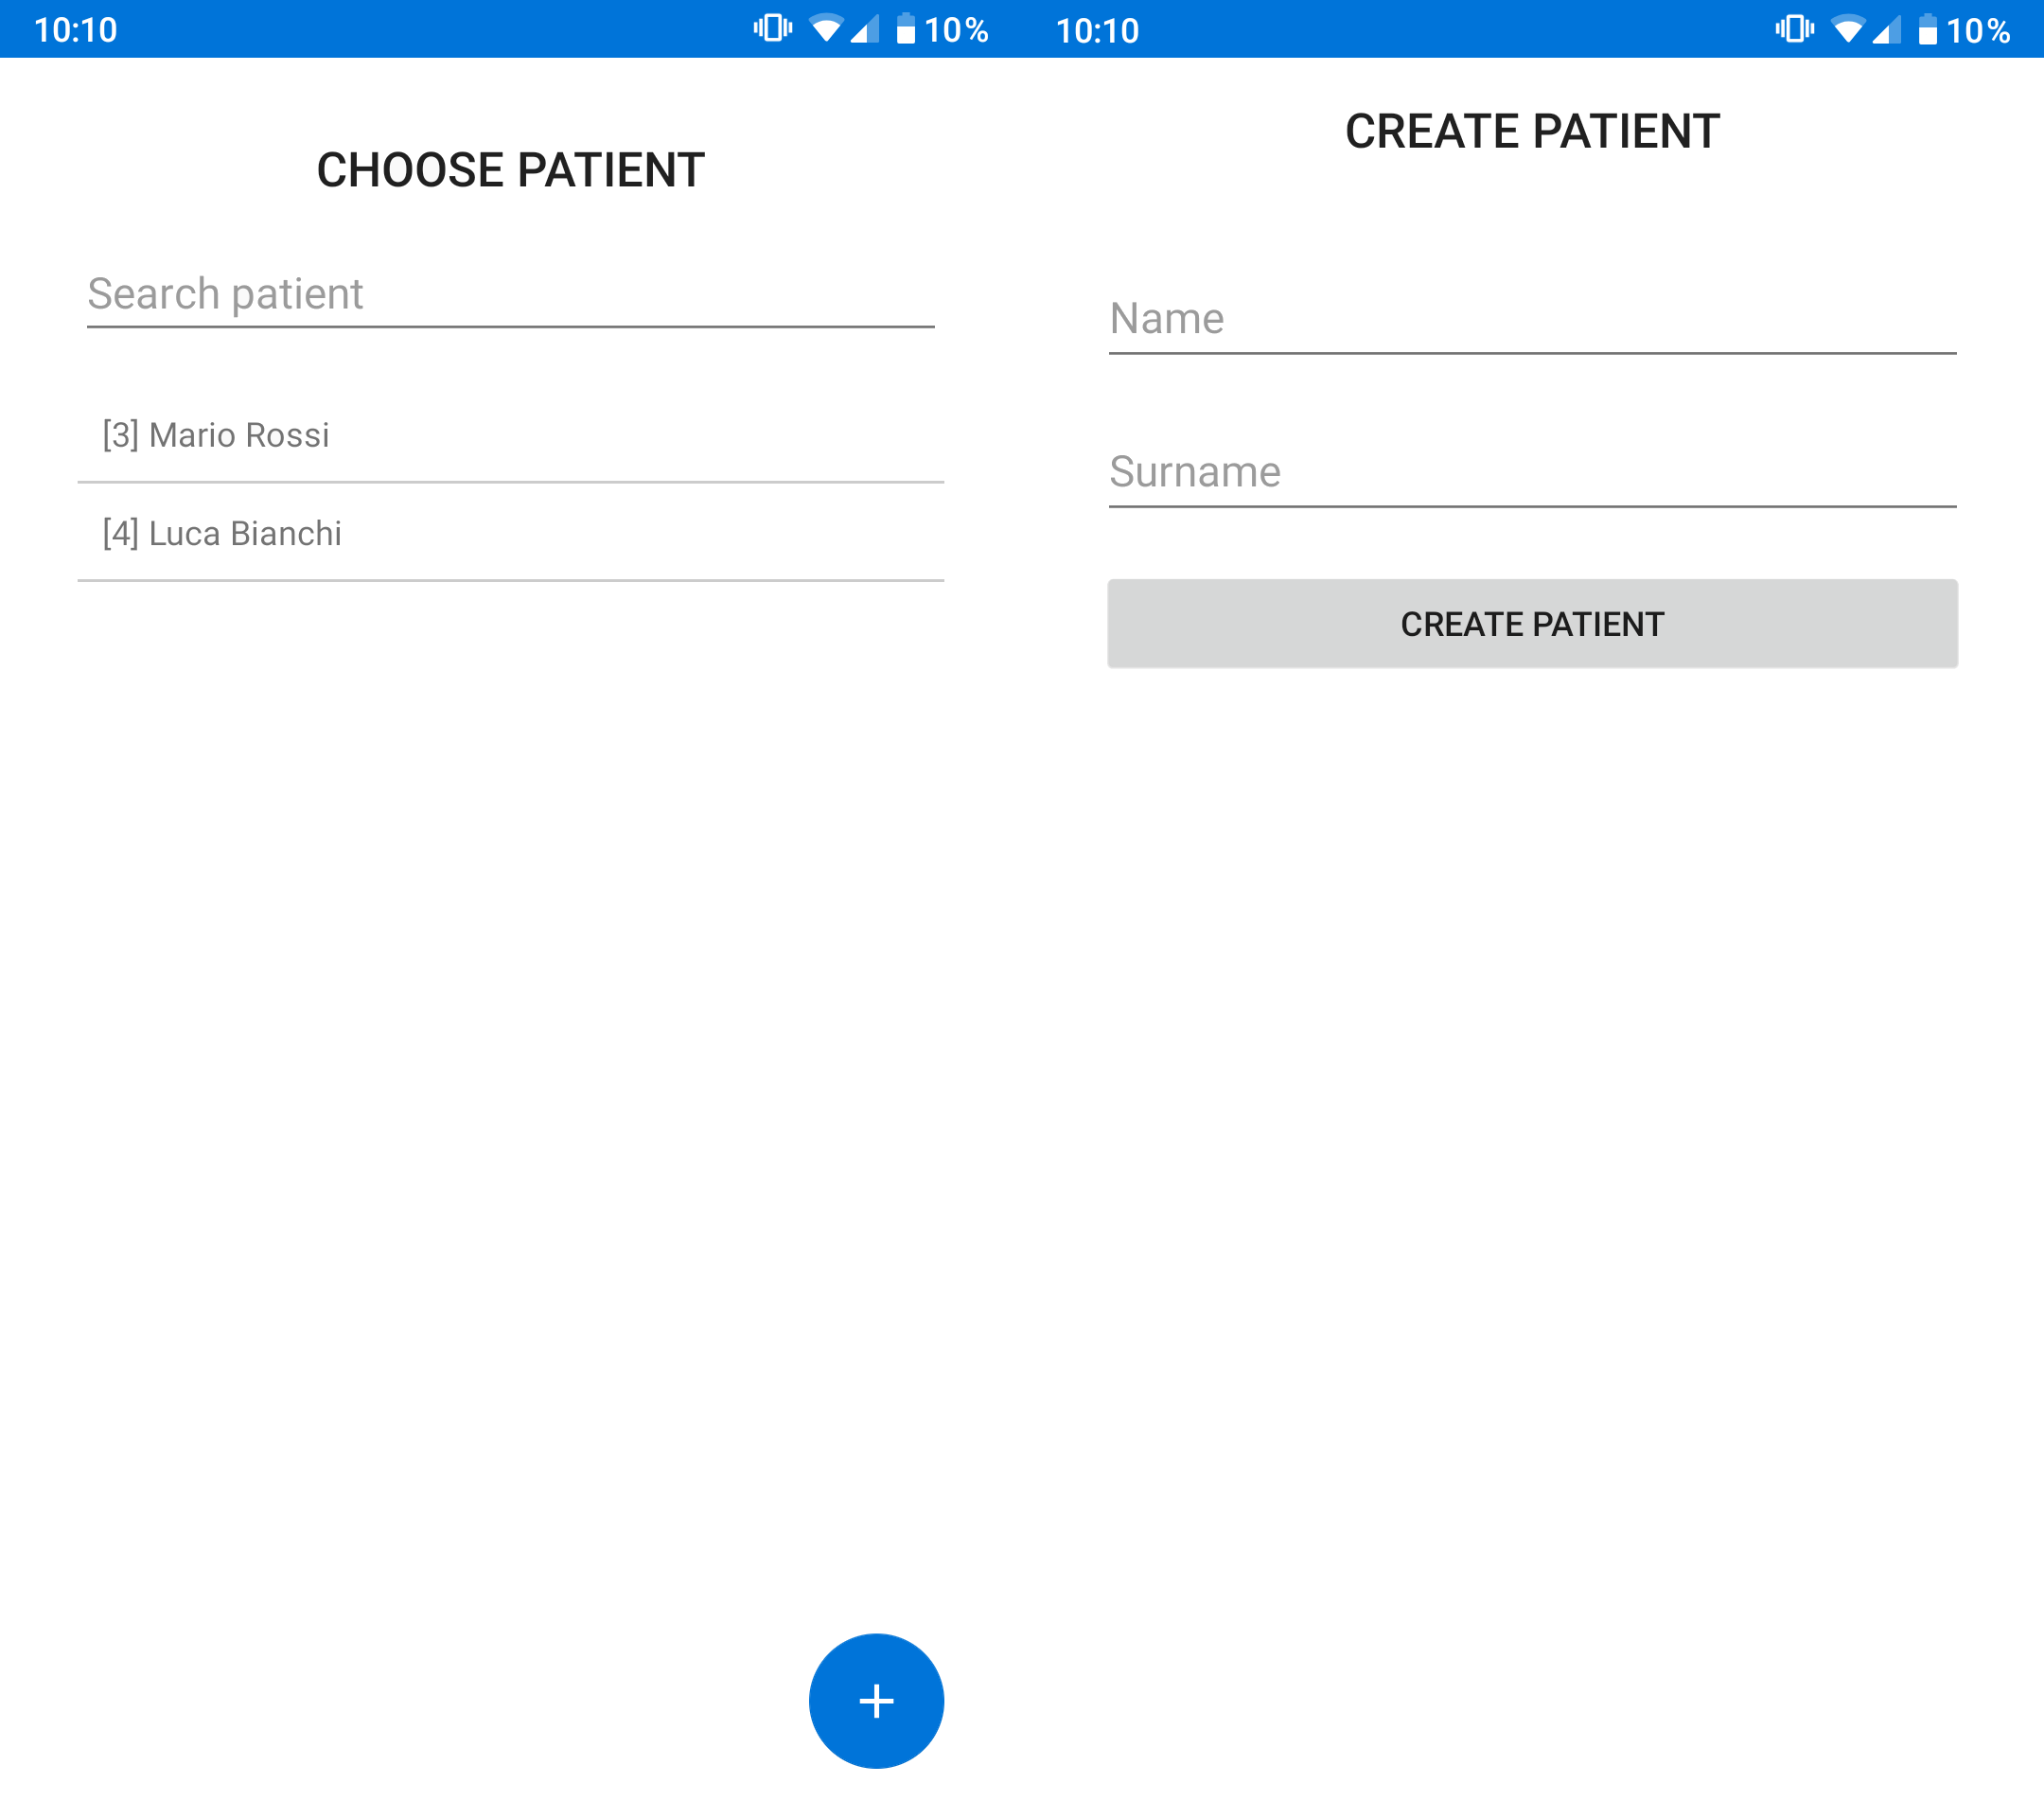
\includegraphics[width=0.70\columnwidth]{images/app_choose_create_patient.png}}
\caption{MainPatient.java, CreatePatient.java}
\label{fig:app_choose_create_patient}
\end{figure}
A questa sezione si accede cliccando il pulsante \textit{choose patient} nel menu del dottore. Nell'attività \textit{MainPatient.java} verrà scaricata automaticamente dalla servlet la lista di tutti i pazienti gestiti dal dottore stampati in questo formato \textit{"[ID] Nome Cognome"}. È presente una barra di ricerca per velocizzare l'individuazione e la selezione di un paziente. 

Selezionando un qualsiasi paziente si ritorna nel menu principale del dottore e verrà visualizzato il paziente appena selezionato; sarà inoltre possibile iniziare il test o vedere i risultati dei test precedentemente ottenuti dal paziente.

Cliccando sul bottone blu si passa all'attività \textit{CreatePatient.java} dove è possibile creare un paziente compilando con nome e cognome (ID automaticamente generato dalla servlet con una numerazione automatica incrementale). Dopo la creazione, il paziente appena creato verrà automaticamente selezionato ritornando nel menu del dottore.

\vfill

\subsection{Test}
\label{subsec:test}
\begin{figure}[H]
\centering
\fbox{\includegraphics[width=0.70\columnwidth]{images/app_test.png}}
\caption{Test.java}
\label{fig:app_test}
\end{figure}
All'apertura del test saranno visualizzate immagini in versione demo (figura \ref{fig:app_test} a sinistra), come si può notare dalla scritta in basso, per far prendere confidenza al paziente del funzionamento del test e dei tasti. In questa modalità le figure sono facilmente visibili anche senza gli occhialini in aiuto del paziente.

Nella parte centrale vengono rappresentate le immagini contenenti le figure presenti nella matrice dei puntini rossi e blu (esistono diversi set di figure selezionabili nelle impostazioni). Nella barra sottostante vi sono le quattro figure candidate a essere soluzione, ovvero uguali all'immagine soprastante; il paziente dovrà selezionare quella che ha visto nell'immagine sopra per proseguire il test con una nuova immagine.

In basso, tra i pulsanti, è descritta la fase del test: la modalità demo (figura \ref{fig:app_test} a sinistra) oppure il livello di disparità dell'immagine visualizzata (figura \ref{fig:app_test} a destra).

\vfill

\newpage

I tasti in grigio sono:
\begin{itemize}
\item \textbf{START TEST}: inizia il test vero e proprio saltando la demo mode; verrà quindi rappresentata l'immagine con il livello di disparità più alto, l'abbinamento più semplice da risolvere (modificabile dalle impostazioni, di default è 12).
\item \textbf{QUIT}: uscita immediata dal test; viene chiesto se si vuole salvare lo stato del test interrotto nei risultati.
\item \textbf{SKIP}: sostituisce l'immagine attuale con un'altra generata in modo casuale, senza nessuna penalizzazione per il punteggio del test.
\end{itemize}

L'algoritmo che sceglie le immagini da visualizzare e le relative disparità è implementato nella libreria e verrà descritto in seguito.

Al termine del test i risultati saranno visualizzati brevemente in una schermata (\textit{TestResults.java}) e saranno automaticamente caricati sulla servlet; nel caso di errore di rete verranno effettuati dei tentativi di ricaricamento dei dati. Tutti i risultati di un paziente sono sempre disponibili nell'attività \textit{Results.java}.

\vfill

\subsection{Results}
\label{subsec:results}
\begin{figure}[H]
\centering
\fbox{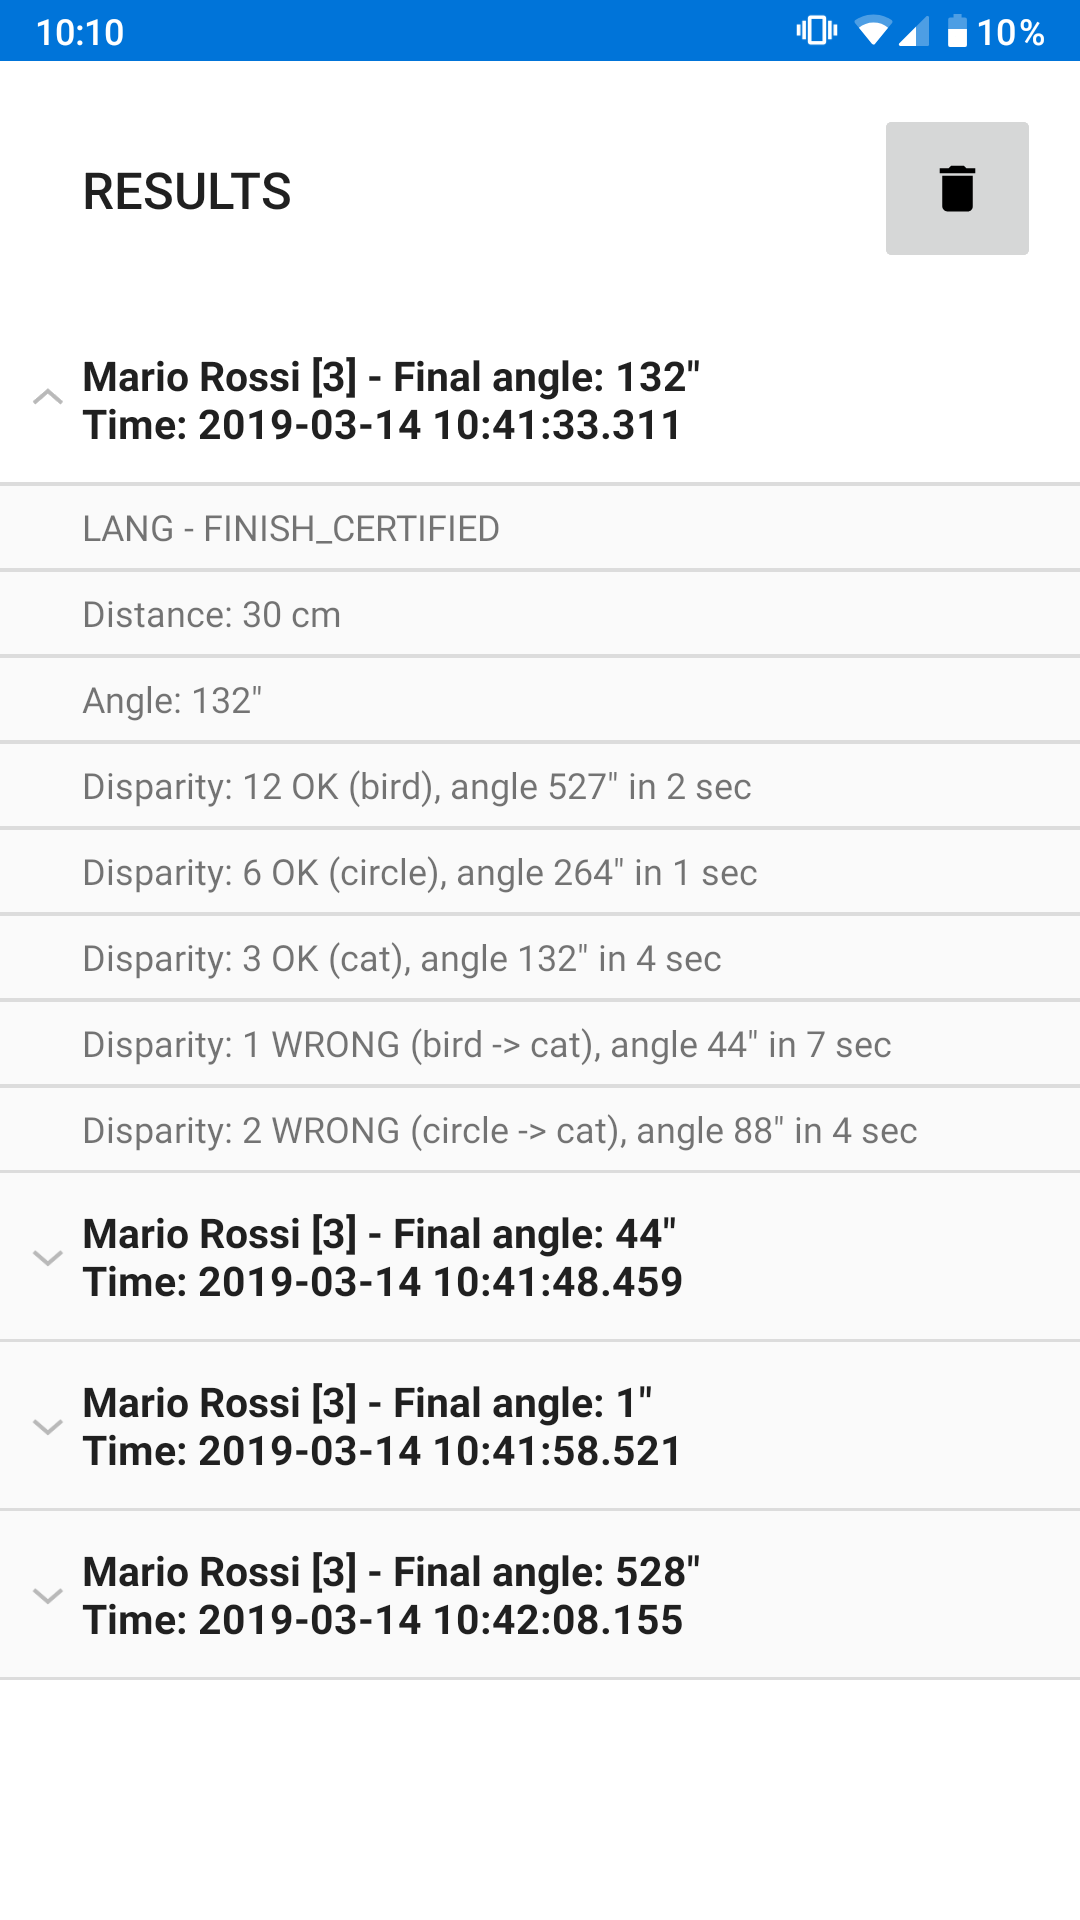
\includegraphics[width=0.35\columnwidth]{images/app_results.png}}
\caption{Results.java}
\label{fig:app_results}
\end{figure}
In questa attività è presente lo storico dei risultati relativi ai singoli test effettuati dallo specifico paziente selezionato. L'elenco è in ordine cronologico e oltre al timestamp è anche indicato anche il \textit{final angle} raggiunto dal paziente.

Espandendo un test specifico cliccandoci sopra, si potranno visualizzare ulteriori dettagli: la certificazione raggiunta dal paziente, la distanza dallo schermo con cui si è effettuato il test, l'angolo finale raggiunto dal paziente e la lista di tutti i tentativi fatti dal paziente indicanti la disparità, la coppia figura selezionata-figura giusta e in quanto tempo il paziente ha effettuato la scelta.

Tenendo premuto su un test specifico è possibile richiedere la sua eliminazione del singolo test dalla servlet, oppure, cliccando il tasto in alto a destra sull'icona del cestino, è possibile richiedere l'eliminazione di tutti i test di quello specifico paziente dalla servlet.

\vfill

\subsection{Settings}
\label{subsec:settings}
\begin{figure}[H]
\centering
\fbox{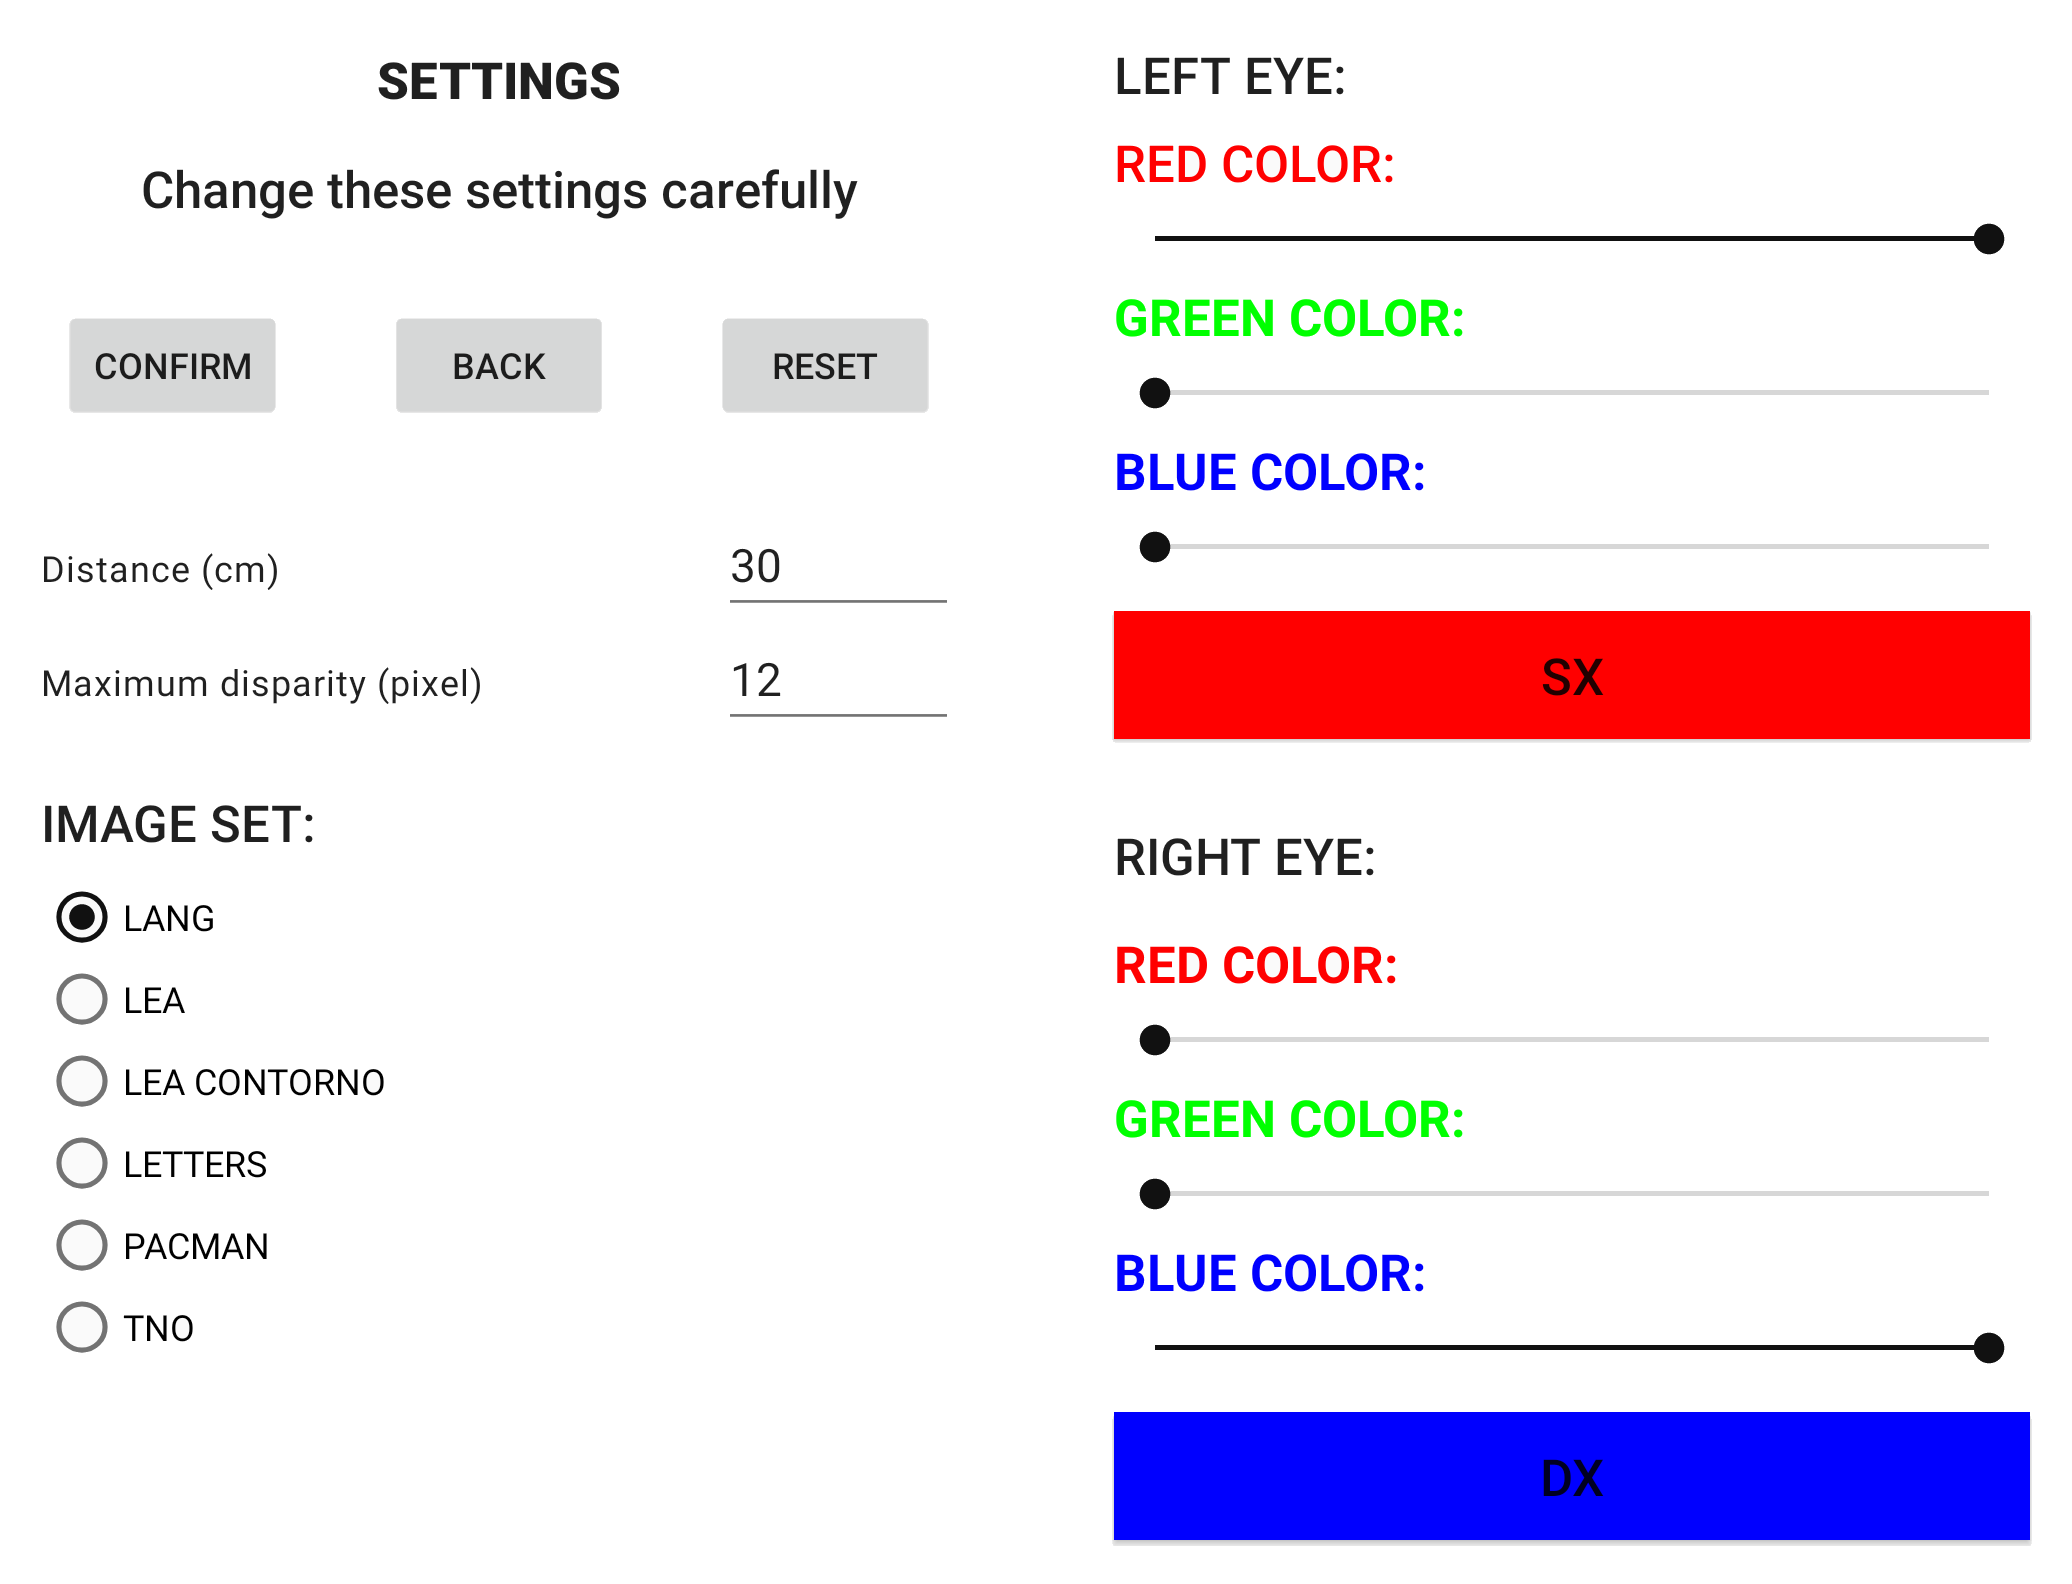
\includegraphics[width=0.70\columnwidth]{images/app_settings.png}}
\caption{Settings.java}
\label{fig:app_settings}
\end{figure}
In questa attività è possibile modificare le impostazioni dell'applicazione. In particolare è possibile modificare la distanza dallo schermo, la disparità massima e il livello iniziale di disparità con cui si inizia il test. La disparità più piccola che bisognerà raggiungere durante il test è fissata per default a 1. In caso di errata resa dei colori dello schermo del cellulare è possibile settare manualmente i colori blu e rosso bilanciando i valori RGB.

Inoltre, è possibile modificare il set di immagini (figura \ref{fig:app_set_images}) che verranno visualizzate durante il test; in ordine dall'alto al basso, da sinistra a desta sono: LANG, LEA, LEA CONTORNO, LETTERS, PACMAN, TNO.

\begin{figure}[H]
\centering
\fbox{
\includegraphics[width=0.50\columnwidth]{images/app_set_images.png}}
\caption{Set di immagini}
\label{fig:app_set_images}
\end{figure}

\vfill

\section{Util activities}
\label{sec:utilactivities}

\subsection{Bitmap}
\label{subsec:bitmap}
\textbf{Activities}: \textit{BitmapBuilder.java, BitmapParallelBuilder.java, SingleBitmapBuilder.java}

Sono tutte classi che lavorano in background che si occupano di creare la matrice formata dai puntini blu/rossi che andranno a comporre l'immagine da visualizzare durante il test.

\subsection{DefaultValues}
\label{subsec:defaultvalues}
\textbf{Activity}: \textit{DefaultValues.java}

In questa classe sono dichiarate tutte le costanti statiche che verranno usate nel codice dalle altre attività e tutti i valori di default delle varie variabili usate nell'applicazione.

Degne di nota sono queste due costanti:

\begin{lstlisting}[language=Java, label=lst:constant, caption={}]
public static final String AUTHORITY = "se4med.unibg.it";
public static final String STEREOTEST = "StereoTest";
\end{lstlisting}

La prima indica l'indirizzo su cui è ospitata la servlet, costante usata durante ogni connessione presente nell'applicazione. La seconda indica l'ID dell'applicazione usato per identificare il nostro progetto tra tutti quelli presenti in 3D4AMB e SE4MED.

\subsection{HashFunction}
\label{subsec:hashfunction}
\textbf{Activity}: \textit{HashFunction.java}

Classe contenente metodi necessari per convertire la password inserita dal dottore durante il login in SHA-256. Viene quindi salvato in SharedPreferences il corrispondente codice SHA-256 generato dalla password che trasmesso come parametro alla servlet a ogni richiesta di un servizio, compreso il login. In questo modo è possibile oscurare la password durante la connessione con la servlet evitando di passare la password in chiaro.

\vfill

\newpage

Il codice della classe HashFunction è il seguente:

\begin{lstlisting}[language=Java, label=lst:sha256, caption={}]
public class HashFunction {
    public static String toSha256(String password) throws NoSuchAlgorithmException {
        MessageDigest md = MessageDigest.getInstance("SHA-256");
        md.update(password.getBytes());
        return bytesToHex(md.digest());
    }

    private static String bytesToHex(byte[] bytes) {
        StringBuilder result = new StringBuilder();
        for (byte byt : bytes)
            result.append(Integer.toString((byt & 0xff) + 0x100, 16).substring(1));
        return result.toString();
    }
}
\end{lstlisting}

\subsection{Other}
\label{subsec:other}
\textbf{Activities}: \textit{Group.java, ListViewAdapter.java, MyExpandableListAdapter.java}

Classi di supporto nella creazione dei menu, delle liste o degli elenchi presenti nell'applicazione.\\

\textbf{Activity}: \textit{Patient.java}

Attività di supporto durante la composizione della tripla \textit{"nome, cognome, ID"} del paziente.

\vfill

\newpage

\section{Dettagli tecnici}
\label{sec:dettaglitecnici}

\subsection{AsyncTask}
\label{subsec:asynctask}

Ogni connessione verso la servlet viene effettuata con un task asincrono (AsyncTask) in modo da evitare il blocco dell'applicazione. Tutte le connessioni seguono un pattern ricorrente e molto simile tra loro; è possibile consultare l'appendice \ref{chap:asynctask} per il codice completo.

\subsection{SharedPreferences}
\label{subsec:sharedpreferences}
Quest'applicazione usa SharedPreferences per salvare i dati riguardanti il dottore, il paziente e le impostazioni.

\begin{lstlisting}[language=Java, label=lst:sharedpreferences, caption={Porzione di codice presa da DefaultValues.java}]
/**
 * SPDOCTOR
 */
public static final String SPDOCTOR = "SPDoctor";
public static final String ACTUAL_DOCTOR_MAIL = "actual_doctor_mail";
public static final String ACTUAL_DOCTOR_PASSWORD = "actual_doctor_password";
public static final String ACTUAL_DOCTOR_NAME = "actual_doctor_name";
public static final String ACTUAL_DOCTOR_SURNAME = "actual_doctor_surname";

/**
 * SPPATIENT
 */
public static final String SPPATIENT = "SPPatient";
public static final String ACTUAL_PATIENT_NAME = "actual_patient_name";
public static final String ACTUAL_PATIENT_SURNAME = "actual_patient_surname";
public static final String ACTUAL_PATIENT_ID = "actual_patient_id";

/**
 * SPSETTINGS
 */
public static final String SPSETTINGS = "SPSettings";
public static final String PREF_DISTANCE = "pref_distance";
public static final String PREF_MAXDISPARITY = "pref_maxdisparity";
public static final String PREF_MINDISPARITY = "pref_mindisparity";
public static final String PREF_IMAGESET = "pref_imageset";
public static final String PREF_OFFSET = "pref_offset";
public static final String PREF_NCORR_TO_NEXTLEVEL = "pref_ncorrtonextlevel";
public static final String PREF_NERR_TOSTOPTEST = "pref_nerrtostoptest";
public static final int DEFAULT_DISTANCE = 30;
public static final int DEFAULT_MAXDISPARITY = 12;
public static final int DEFAULT_OFFSET = 1;
public static final int DEFAULT_NCORR_TONEXTLEVE = 1;
public static final int DEFAULT_NERR_TOSTOPTEST = 3;
public static final ImageShape.ImageSet DEFAULT_IMAGESET = ImageShape.ImageSet.LANG;
public static final int POSSIBLECHOICES = 4; // Possible choices in Test
\end{lstlisting}

%%%%% SERVLET %%%%%
\chapter{Servlet}
\label{chap:servlet}

\section{Introduzione alla servlet}
\label{sec:introduzioneallaservlet}
La servlet ospitata all'indirizzo \textit{se4med.unibg.it/home} è condivisa tra tutti i progetti universitari e mette a disposizione una serie di servizi atti sia all'autenticazione delle varie applicazioni che al salvataggio di dati in un database centrale. La servlet è scritta in Java, noi abbiamo usato l'ambiente di sviluppo Eclipse Maven \cite{eclipse} per implementare nuovi metodi che la nostra applicazione richiedeva. Oltre alla servlet abbiamo lavorato anche sul database usando MySQL \cite{mysql}.\\

\begin{table}[]
\centering
\begin{tabular}{lllll}
\toprule
\textbf{Servlet} &  se4med.unibg.it/home\\
\textbf{Tools} & Eclipse Maven, MySQL\\
\bottomrule
\end{tabular}
\caption{Dettagli servlet \label{t:1}}
\end{table}

Abbiamo anche creato un account di prova su \textit{se4med.unibg.it/home} per un dottore dove effettuare tutti i test necessari:\\

\begin{table}[]
\centering
\begin{tabular}{lllll}
\toprule
\textbf{Account} &  doctorsat@mail.com\\
\textbf{Password} & doctorsat\\
\bottomrule
\end{tabular}
\caption{Credenziali dell'account di prova \label{t:1}}
\end{table}

\newpage

\section{Database}
\label{sec:database}
Il database connesso alla servlet è molto vasto, le tabelle usate dal nostro progetto sono quelle rappresentate in figura \ref{fig:database}.

\begin{figure}[H]
\centering
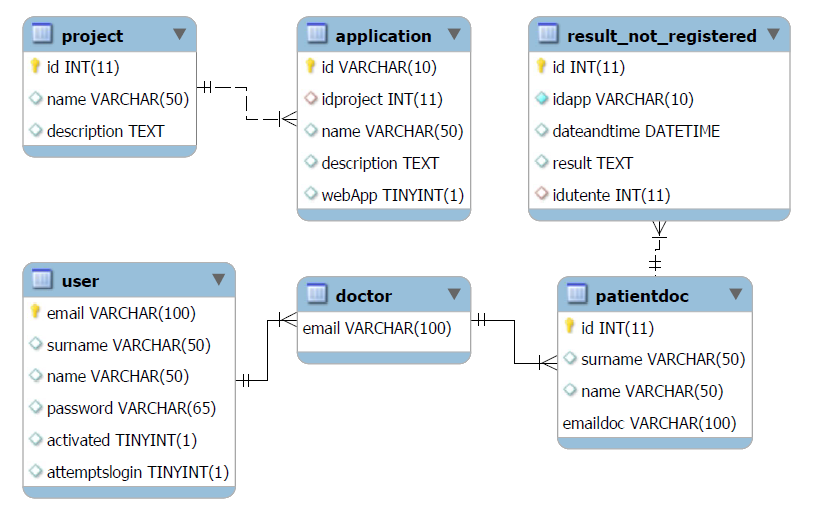
\includegraphics[width=0.9\columnwidth]{images/database.png}
\caption{Database della servlet}
\label{fig:database}
\end{figure}

\begin{itemize}
\item Tabella \textbf{project}: elenca tutti i progetti presenti nel database, tra i quali il nostro denominato \textit{Stereo Acuity Test}.
\item Tabella \textbf{application}: elenca tutte le applicazioni create, riferite a un particolare progetto; la nostra applicazione ha come \textit{idapp} il valore \textit{StereoTest}.
\item Tabella \textbf{user}: elenca tutti gli utenti che hanno effettuato la registrazione.
\item Tabella \textbf{doctor}: elenca tutti i dottori registrati.
\item Tabella \textbf{patientdoc}: elenca tutti i pazienti gestiti da uno specifico dottore.
\item Tabella \textbf{result\_not\_registered}: elenca tutti i risultati dei test effettuati dai pazienti; i dati sono salvati in formato JSON\footnote{JavaScript Object Notation} \cite{json}.
\end{itemize}

\newpage

Nella servlet, per scrivere il codice necessario per interrogare e modificare il database, ci siamo serviti di JOOQ\footnote{Java Object Oriented Quering} \cite{jooq}, una libreria software leggera per il database-mapping in Java che fornisce un linguaggio specifico di dominio per costruire query da classi generate da uno schema di database.

\section{Servizi}
\label{sec:servizi}
Nella servlet abbiamo implementato questi nuovi servizi usati dall'applicazione:

\begin{itemize}
\item Servizio \textbf{authenticate\_doctor\_ns\_action}: autenticazione del dottore, usata dall'applicazione nel login form iniziale.
\item Servizio \textbf{getpatientdoclist\_action}: ritorna la lista dei pazienti gestiti dal dottore specifico in formato \textit{"nome, cognome, id"}.
\item Servizio \textbf{createpatientdoc\_action}: crea un paziente con nome, cognome e id autogenerato e lo associa al dottore.
\item Servizio \textbf{deletepatientdoc\_action}: cancella lo specifico paziente richiesto dal dottore.
\item Servizio \textbf{storeresults\_not\_registered\_action}: salvataggio del risultato finale del singolo test effettuato dal paziente.
\item Servizio \textbf{getresults\_not\_registered\_action}: ritorna la lista di tutti i risultati dei test di uno specifico paziente associato al dottore.
\item Servizio \textbf{deleteresults\_all\_action}: cancella tutti i risultati dei test di uno specifico paziente associato al dottore.
\item Servizio \textbf{deleteresult\_single\_action}: cancella il singolo test selezionato di uno specifico paziente associato al dottore.
\end{itemize}

\newpage

Le risposte all'interrogazione della servlet sono in formato JSON e nell'applicazione è possibile estrarre il contenuto e l'informazione desiderata.
Di seguito sono elencate tutte le interfacce usate per l'interrogazione e la modifica del database usando JOOQ con i rispettivi parametri passati durante la richiesta:

\begin{lstlisting}[language=Java, label=lst:parameters, caption={Interfacce per l'interrogazione e la modifica del database}]
String getNameSurnameDoctor(String emaildoc, String password, String idapp);

ArrayList<String> getPatientDocList(String emaildoc, String password, String idapp);

int createPatientDoc(String emaildoc, String password, String name, String surname, String idapp);

int deletePatient(String emaildoc, String password, String idpatient, String idapp);

int storeResultsNotRegistered(String emaildoc, String password, String idpatient, String idapp, Timestamp datetime,
			String result);

ArrayList<String> getResultsNotRegistered(String emaildoc, String password, String idpatient, String idapp);

int deleteResultsAll(String emaildoc, String password, String idpatient, String idapp);

int deleteResultSingle(String emaildoc, String password, String idpatient, String idapp, String results);
\end{lstlisting}

%%%%% LIBRERIA %%%%%
\chapter{Libreria}
\label{chap:libreria}

\section{Introduzione alla libreria}
\label{sec:introduzioneallalibreria}
La libreria per lo \textit{Stereo Acuity Test} è stata modificata implementando il PEST\footnote{Parameter Estimation by Sequential Testing}, un nuovo algoritmo di calcolo dei livelli di profondità dell'immagine che permette in pochi passaggi di trovare la profondità massima raggiungibile dal paziente. Questa libreria è usata dall'applicazione per determinare la sequenza di immagini con la relativa disparità mostrate durante il test; tuttavia essa potrà essere usata in futuro da qualsiasi altra applicazione che necessiterà dell'algoritmo PEST. Per modificare la libreria scritta in Java abbiamo usato l'ambiente di sviluppo Eclipse Maven \cite{eclipse}.\\

\begin{table}[]
\centering
\begin{tabular}{lllll}
\toprule
\textbf{Library} &  lib3dsat\_pest.jar\\
\textbf{Tools} & Eclipse Maven\\
\bottomrule
\end{tabular}
\caption{Dettagli libreria \label{t:1}}
\end{table}

Per comprendere l'algoritmo ci siamo basati sia su un estratto di Alex Pentlando \textit{"Maximum likelihood estimation: The best PEST"} \cite{pestalex} che su un articolo di Neil Carter \textit{"Parameter Estimation by Sequential Testing"} \cite{pestneil}.

\newpage

\section{PEST (Parameter Estimation by Sequential Testing)}
\label{sec:pest}
L'\textbf{algoritmo PEST} si basa su una procedura descritta da M. M. Taylor e C. Douglas Creelman in \textit{"PEST: Efficient Estimates on Probability Functions"} \cite{pest}. In esso sono definite un insieme di regole da seguire per settare e impostare la difficoltà di un determinato processo, con lo scopo di riuscire a rilevare il più velocemente possibile il livello a cui le performance tendono in maniera predefinita. In maniera formale si sostiene che: dati dei segnali con determinate proprietà (variabili indipendenti) si deve ricercare e regolare la precisione delle performance da sottoporre a seconda dei risultati ottenuti (variabili dipendenti).

Nel caso di Taylor e Creelman il test riguardava alcuni partecipanti sui quali furono testate le capacità di ascolto di una varietà di suoni. Il test veniva considerato corretto con una soglia del 25\%, ovvero doveva essere riconosciuto dai partecipanti entro il 75\% delle volte che veniva eseguito. L'obiettivo era capire la velocità del ragionamento mentale che portava a riconoscere il suono come risposta a stimoli ripetuti. Il test venne svolto per risposta diretta sia per selezione tra un numero predefinito di opzioni. A seconda dell'esito della risposta e del tempo di risposta (indice di accuratezza e precisione) il livello veniva cambiato per avere un processo più difficile o viceversa. Il test si concludeva quando una serie di prove rimaneva costante su un certo livello che venne chiamato "step" o "block".

L'algoritmo PEST si rivelò molto efficiente nel riuscire a individuare il livello di performance dei partecipanti con il minimo numero di prove possibile. La sua efficienza è dovuta alle regole che governano la scelta del livello successivo da sottoporre sulla base degli esiti delle risposte precedenti.

Gli studi di Taylor e Creelman del 1967 furono portati avanti da diversi studiosi e furono sviluppate diverse versioni del PEST tra le quali annoveriamo quella di Findlay nel 1978, la cui formula è presente in figura \ref{fig:formula_findlay}.

\begin{figure}[H]
\centering
\fbox{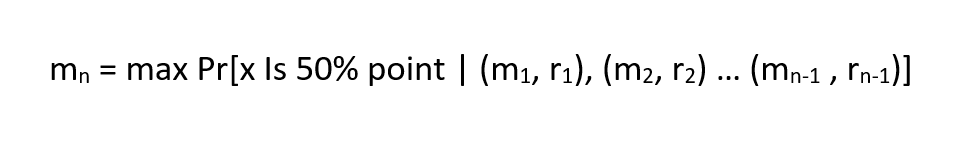
\includegraphics[width=0.70\columnwidth]{images/formula_findlay.png}}
\caption{Formula di Findlay}
\label{fig:formula_findlay}
\end{figure}

La lettera m rappresenta la variabile indipendente da misurare/impostare e come pedice è indicata l'i-esima misurazione svolta. La r corrisponde al risultato della prova e può essere o +1 se corretta o  -1 se errata. Il valore 50\% indica la verosimiglianza che si vuole ottenere.

\section{Studio qualitativo dell'algoritmo}
\label{sec:studioqualitativodellalgoritmo}
In questo paragrafo ci addentreremo negli studi di Taylor e Creelman e in particolare sull'analisi del loro test per certificare i vantaggi che questo algoritmo può apportare.

Il PEST monitora le performance dei partecipanti con una semplice operazione: il calcolo del rapporto tra il numero di risposte corrette date da un partecipante e il totale delle prove; in questo modo si ottiene il punteggio (\textbf{score}) del partecipante che varierà tra zero (tutte risposte sbagliate) e 1 (tutte risposte corrette). Esso viene confrontato con la precisione (\textbf{accuracy}) richiesta dal test e da questo confronto si può prendere una scelta sul livello successivo da sottoporre. La precisione è un parametro molto rilevante che è già preimpostato prima del test: un'alta precisione implica una maggior difficoltà nello svolgere il test e viceversa. Un altro parametro è la deviazione (\textbf{deviation limit}), che previene che ci siano cambiamenti troppo repentini tra un livello e il successivo. Quest'ultima verrà molto utile nei casi particolari come per esempio nel primo livello dove a seconda dell'esito si avrà uno score massimo=1 o minimo=0.

Per studiare qualitativamente l'algoritmo useremo dei \textbf{grafici} che permettano di analizzare la relazione che intercorre tra l'andamento delle risposte corrette e il susseguirsi delle prove con i relativi livelli di difficoltà (rispettivamente fissati sull'asse delle ordinate e delle ascisse).

Nella prima coppia di grafici (vedi figura \ref{fig:pest_acc75}) analizziamo come varia l'algoritmo PEST in funzione della deviazione standard. La banda verde indica il range di valori nel quale non è richiesto un cambiamento di difficoltà della prova. Con i punti rossi e blu indichiamo rispettivamente i casi limite in cui il partecipante risponde rispettivamente in maniera errata o corretta a tutte le prove sottoposte. Confrontando i grafici notiamo che un aumento della deviazione standard relativamente piccolo diminuisce il range in cui è richiesto al PEST un cambio di livello difficoltà. In altri termini la deviazione standard è una grandezza direttamente proporzionale alla stabilità con quest'ultima intesa come mantenimento costante del livello tra step successivi.

\begin{figure}[H]
\centering
\fbox{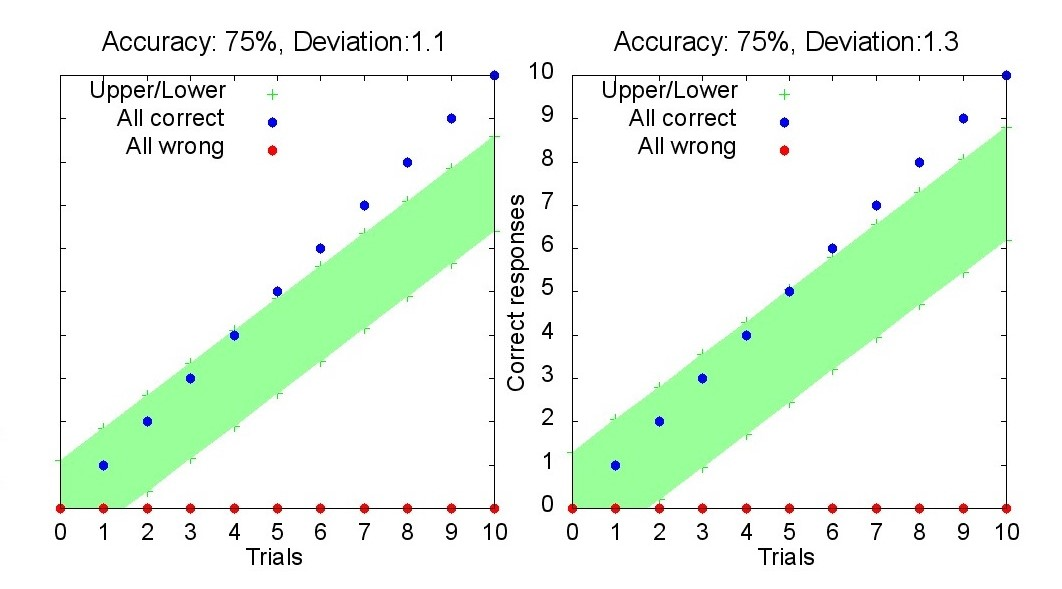
\includegraphics[width=0.70\columnwidth]{images/pest_acc75.png}}
\caption{Grafici con precisione 75\%}
\label{fig:pest_acc75}
\end{figure}

Negli ultimi due grafici (vedi figura \ref{fig:pest_acc85}) invece valutiamo gli effetti causati da un aumento del 10\% di precisione. La banda  in cui è richiesta una difficoltà costante risulta essere più aderente alle risposte corrette. In genere un aumento di accuratezza provoca nel caso di risposta corretta una nuova domanda molto più difficile e viceversa in caso di risposta errata una nuova domanda molto più facile. Sempre in termini di stabilità come precedentemente definita, possiamo affermare che la precisione risulta essere inversamente proporzionale alla stabilità.

\begin{figure}[H]
\centering
\fbox{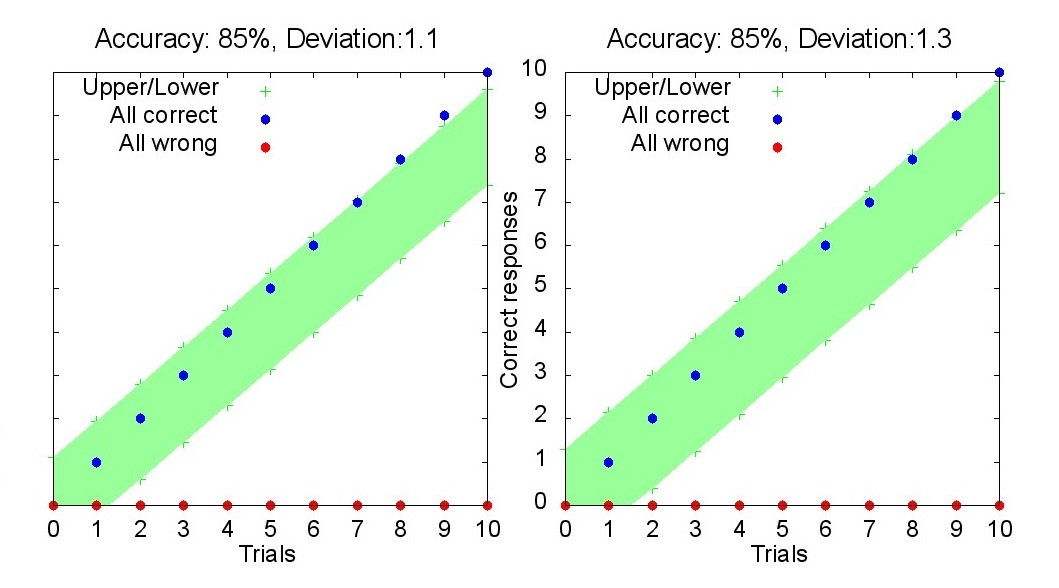
\includegraphics[width=0.70\columnwidth]{images/pest_acc85.png}}
\caption{Grafici con precisione 85\%}
\label{fig:pest_acc85}
\end{figure}

\vfill

\newpage

\section{Implementazione dell'algoritmo}
\label{sec:implementazionedellalgoritmo}

Abbiamo implementato due algoritmi di PEST entrambi testati con i relativi casi di test. Il primo algoritmo si trova nella classe \textit{PestDepthCertifierOld} e segue di pari passo le regole definite da Taylor e Creelman nel loro saggio.
Tuttavia, nella nostra applicazione è stato implementato un'evoluzione di tale algoritmo con accorgimenti e modifiche funzionali atte all'adattarsi ai nostri requisiti. Questo algoritmo si trova nella classe \textit{PestDepthCertifier} e verrà gradualmente descritto in questo capitolo.

Ad ogni livello di disparità è associato un angolo che indica la profondità dell'immagine blu/rossa sullo schermo. 

\begin{osservazione}\normalfont
I numeri dei livelli sono inversamente proporzionali alla profondità dell'immagine e quindi alla difficoltà del livello. Il livello con maggiore profondità, quindi il più difficile da superare, è il livello 1.
\end{osservazione}

Un insieme definito da due variabili \textit{leftLimit} e \textit{rightLimit}, che indicano rispettivamente il limite sinistro e destro di tale insieme, è necessario per racchiudere all'interno il valore corrente della disparità di un determinato livello (variabile \textit{currentDepth}).

\begin{osservazione}\normalfont
\textit{leftLimit > currentDepth > rightLimit}
\end{osservazione}

Per istanziare la classe \textbf{PestDepthCertifier} (codice \ref{lst:pestdepthcertifier}) è richiesto un solo argomento: \textit{initDepth = maxDepth} che è il livello iniziale, ossia il più semplice da superare che è anche il massimo livello nel test. Il livello iniziale è impostato a 12 per default ma può essere cambiato nelle impostazioni dell'applicazione dal dottore; il livello minimo, quello più complesso da raggiungere, è fissato a 1. Secondo quanto visto nell'ultima osservazione viene inizializzato l'insieme ponendo \textit{leftLimit = initDepth} e \textit{rightLimit = 1}.

Viene istanzato anche un'array chiamato \textit{vector} con dimensione uguale al numero di livelli del test (\textit{initDepth}) che permetterà di salvare le risposte date dal paziente nel seguente modo: inizialmente i suoi elementi saranno posti tutti a zero (ad esempio con \textit{initDepth = 12} avremo [0,0,0,0,0,0,0,0,0,0,0,0]). Ogni posizione dell’array corrisponde ad un livello: le risposte corrette sono registrate sommando un 1 nella specifica posizione dell'array, mentre le risposte errate sono salvate sottraendo un 1.

La variabili \textit{chance}  e \textit{weight} verranno spiegate in seguito.

\begin{lstlisting}[language=Java, label=lst:pestdepthcertifier, caption={Classe PestDepthCertifier}]
public PestDepthCertifier(int initDepth) {
	certifierStatus = new CertifierStatus();

	if (initDepth >= 1)
		certifierStatus.currentDepth = initDepth;
	else
		throw new IllegalArgumentException();

	maxDepth = initDepth;
	leftLimit = initDepth;
	rightLimit = 1;
	chance = 1;
	vector = new int[initDepth];
	weight = 1;
	partone = true;

	certifierStatus.currentResult = CONTINUE;
}
\end{lstlisting}

Prima dell'avvio del test si avrà una demo del livello con disparità \textit{initDepth} per far prendere familiarità con i comandi ai pazienti e successivamente inizierà il test vero e proprio.

Il metodo \textbf{computeNextDepth} (codice \ref{lst:computenextdepth}) di tipo void riceve come argomento l'esito della risposta data dal paziente ad un determinato livello e procede a computare il livello successivo da sottoporre al paziente. Nel caso in cui si sia raggiunto il livello finale o l'algoritmo riconosca il livello di performance del paziente, si procede a stampare la certificazione.

L’algoritmo è composto da due macro-fasi in successione. 

La prima fase (\textbf{PART ONE}) ha lo scopo di individuare con il minor numero di prove possibile un range di due valori in cui è molto alta la probabilità che vi si trovi il livello di performance del paziente. 

La seconda fase (\textbf{PART TWO}) partendo dal range trovato nella fase precedente permette di determinare precisamente il livello del paziente.

\newpage

\begin{lstlisting}[language=Java, label=lst:computenextdepth, caption={Metodo computeNextDepth}]
void computeNextDepth(DepthCertBase.Solution solution) {
	int savedCurrentDepth = certifierStatus.currentDepth;

	// PART ONE
	// Quickly and approximately identify the range in which the level can be contained
	if (partone && (solution != DepthCertBase.Solution.NULL)) {
		System.out.print("[PART ONE]");

		if (solution == DepthCertBase.Solution.WRONG && chance > 0 && certifierStatus.currentDepth == maxDepth) {
			// First wrong attempt to maxDepth
			chance--;
		} else if (solution == DepthCertBase.Solution.WRONG && chance == 0
				&& certifierStatus.currentDepth == maxDepth) {
			// Second wrong attempt to maxDepth
			certifierStatus.currentResult = FINISH_NOT_CERTIFIED;
		} else if (solution == DepthCertBase.Solution.RIGHT) {
			leftLimit = certifierStatus.currentDepth;

			// Numerical rounding (Floor: round down)
			value = ((double) leftLimit + rightLimit) / 2;
			nextDepth = (int) (Math.floor(value));

			certifierStatus.currentDepth = nextDepth;
			vector[leftLimit - 1] += 1;

			if ((leftLimit - rightLimit) == 1) {
				partone = false;
				nextDepth = rightLimit;
				certifierStatus.currentDepth = nextDepth;
				
				// Weight because the rightLimit was wrong
				if (rightLimit != 1)
					weight = weight*3;
			}
		} else if (solution == DepthCertBase.Solution.WRONG) {
			rightLimit = certifierStatus.currentDepth;

			// Numerical rounding (Ceil: round up)
			value = ((double) leftLimit + rightLimit) / 2;
			nextDepth = (int) (Math.ceil(value));

			certifierStatus.currentDepth = nextDepth;
			vector[rightLimit - 1] -= 1;

			if ((leftLimit - rightLimit) == 1) {
				partone = false;
				nextDepth = rightLimit;
				certifierStatus.currentDepth = nextDepth;
				
				// Weight because the rightLimit was wrong
				if (rightLimit != 1)
					weight = weight*3;
			}
		}
		
		// PART TWO
		// Focus on the lower level identified [nextDepth = rigthLimit] until it reaches
		// a +2 that certifies the level, or a -2 that shift to an easier level
		// (nextDepth++). Added weight to avoid loop like [OK | NO | OK | NO]
	} else if (!partone && (solution != DepthCertBase.Solution.NULL)) {
		System.out.print("[PART TWO]");

		if (solution == DepthCertBase.Solution.RIGHT) {
			vector[nextDepth - 1] += 1;
			certifierStatus.currentDepth = nextDepth;
		} else if (solution == DepthCertBase.Solution.WRONG) {
			// Subtract with weight
			vector[nextDepth - 1] -= weight;
			weight = weight * 3;
			certifierStatus.currentDepth = nextDepth;
		}

		// Vector control and maxDepth control
		if (vector[nextDepth - 1] >= 2) {
			// Reached the certification
			certifierStatus.currentResult = FINISH_CERTIFIED;
			certifierStatus.currentDepth = nextDepth;
		} else if ((vector[nextDepth - 1] <= -2) && (nextDepth < maxDepth)) {
			// Shift the nextDepth and reset weight
			nextDepth++;
			weight = 1;
			certifierStatus.currentDepth = nextDepth;
		} else if ((vector[nextDepth - 1] <= -2) && (nextDepth == maxDepth)) {
			// Returned to the initial maxDepth without certification
			certifierStatus.currentResult = FINISH_NOT_CERTIFIED;
			certifierStatus.currentDepth = nextDepth;
		}
	} else {
		System.out.print("[NULL (SKIP BUTTON)]");
		assert solution == DepthCertBase.Solution.NULL;
	}
}
\end{lstlisting}

\subsection{PART ONE}
\label{subsec:part one}

Nella prima fase, ad ogni step l'algoritmo conosce il valore di \textit{currentDepth} e riceve l'esito della risposta data dal paziente sulla base della figura scelta:

\begin{itemize}
\item \textbf{RIGHT}: come conseguenza ad una risposta corretta del paziente si aggiorna il limite sinistro con il livello corrente appena superato e si calcola il livello successivo come la media tra il limite sinistro e il limite destro con arrotondamento per difetto.

\textit{leftLimit = currentDepth}
\item \textbf{WRONG}: come conseguenza ad una risposta errata del paziente si aggiorna il limite destro con il livello corrente appena sbagliato e si calcola il livello successivo come la media tra il limite sinistro e il limite destro con arrotondamento per eccesso.

\textit{rightLimit = currentDepth}

\item \textbf{NULL (SKIP)}: non si esegue nulla, verrà riproposta un'altra immagine di pari livello di disparità.
\end{itemize}

Le tre casistiche sono mutuamente esclusive e portano ad una riduzione progressiva dell'insieme. Nel momento in cui l'insieme si riduce a due livelli consecutivi (\textit{leftLimit - rightlimit == 1}) la prima fase termina. Notiamo che ad ogni step, prima di effettuare la decisione del livello successivo, l'algoritmo salva l'esito della risposta data dal paziente nell'array \textit{vector}.

\subsection{PART TWO}
\label{subsec:part two}

La seconda fase ha inizio con la terminazione della prima; poniamo la variabile \textit{nextDepth = rightLimit} in modo che il prossimo livello da testare sarà il limite destro. Il valore del livello \textit{rightLimit} nell'array avrà valore -1:  la motivazione risiede nel fatto che nella prima parte dell'algoritmo il limite destro viene aggiornato solo in presenza di una risposta errata e, viceversa, il limite sinistro viene aggiornato solo in conseguenza di una risposta corretta. Inoltre la variabile \textit{weight} sarà pari a 3 avendo già sbagliato quel livello nella prima parte dell'algoritmo. Un'eccezione è quando \textit{rightLimit = 1}, in questo caso il valore nell'array è 0 e la variabile \textit{weight} sarà pari a 1 perchè non è stato mai commesso un errore sul livello 1.

Una serie di tre risposte corrette senza errori porterà a terminare l’algoritmo restituendo quel livello, aumentando a ogni step di 1 il valore dell'array fino a raggiungere 2 che provoca un'uscita certificata. Un eventuale errore provocherà l’esclusione di quel livello e l'inizio di un processo ricorsivo governato dalle seguenti regole:

\begin{itemize}
\item In caso di risposta corretta verrà sommato 1 alla posizione \textit{(i - 1)} dell'array, corrispondente al livello \textit{nextDepth} sottoposto al paziente.

\textit{vector[nextDepth - 1] += 1;}

\item In caso di risposta errata verrà sottratto \textit{weight} alla posizione \textit{(i - 1)} dell'array, corrispondente al livello \textit{nextDepth} sottoposto al paziente. In particolare al primo errore la variabile \textit{weight} avrà valore 1, mentre ad ogni errore successivo avrà valore (\textit{weight} * 3). Facendo pesare maggiormente i successivi errori evitiamo di entrare in una situazione di loop causata dal paziente che alterna una risposta giusta a una sbagliata. 

\textit{vector[nextDepth - 1] -= (1 * weight);}

\textit{weight = weight * 3;}

\item Nel caso in cui la posizione \textit{(i - 1)} dell'array assumesse valore maggiore o uguale a 2, il livello \textit{nextDepth} viene certificato, ossia è stato superato correttamente almeno due volte.

\textit{vector[nextDepth - 1] >= 2}

\item Nel caso in cui la posizione \textit{(i - 1)} dell'array assumesse valore minore o uguale a -2, la variabile \textit{nextDepth} viene incrementata permettendo di sottoporre al paziente un livello più semplice; inoltre viene resettata a 1 la variabile \textit{weight}.

\textit{vector[nextDepth - 1] <= -2}

\textit{nextDepth++;}

\textit{weight = 1;}

\end{itemize}

Un ulteriore controllo viene effettuato sulla variabile \textit{nextDepth} in modo tale che non venga incrementata oltre il livello iniziale \textit{initDepth = maxDepth}.\\

Per gestire la terminazione, quindi la certificazione del livello raggiunto o meno dal paziente, è necessaria la variabile \textit{certifierStatus.currentResult} che può assumere tre possibili stati:

\begin{itemize}
\item \textbf{FINISH\_CERTIFIED}: l'algoritmo riconosce di aver individuato la performance (profondità) raggiunta dal paziente. La variabile \textit{nextDepth} conterrà il livello raggiunto dal paziente.

\item \textbf{CONTINUE}: sono necessarie ulteriori prove per stabilire il livello finale.

\item \textbf{FINISHED\_NOT\_CERTIFIED}: l'algoritmo termina il test senza riconoscere la certificazione. Avviene nei seguenti casi:

Durante la \textbf{prima fase}, se il paziente ha sbagliato consecutivamente le prime due risposte i cui livelli sono entrambi settati alla profondità iniziale; non avendo risposto a nessuna domanda nel modo corretto il test termina senza la certificazione. Il controllo avviene tramite la variabile \textit{chance} inizializzata a 1 che viene decrementata solo nel caso in cui venga sbagliato il livello iniziale. Quindi al secondo errore la variabile \textit{chance} avrà valore 0 e provocherà l'uscita non certificata.

\textit{rightLimit == currentDepth \& chance == 0}

Durante la \textbf{seconda fase}, a seguito di numerosi errori consecutivi e livelli sempre più facili sottoposti progressivamente, il paziente non è stato in grado di saper risolvere nemmeno il livello massimo (iniziale) nonostante nella prima fase l'abbia risolto correttamente. Nessun livello può essere certificato.

\textit{(vector[nextDepth - 1] <= -2) \&\& (nextDepth == maxDepth)}

\end{itemize}

\newpage

\section{Testing dell'algoritmo}
\label{sec:testingdellalgoritmo}
La totalità dei casi di test svolti si trova nella classe \textbf{PestDepthCertifierTest}. In questa sezione illustreremo alcuni scenari significativi con \textit{initDepht}=12, ovvero con 12 livelli che vanno da 12 a 1.
La validità dei casi di test è stata inoltre certificata con l'uso del plugin per Eclipse \textit{codecover} \cite{codecover} che ha verificato la copertura dei casi di test in relazione al codice dell'algoritmo.

Una struttura di test in generale ha inizio con la creazione di una classe di tipo \textbf{PestDepthCertifier} e contiene più invocazioni del metodo \textbf{checkGoTo} che ha questa struttura:

\begin{lstlisting}[language=Java, label=lst:checkgoto, caption={Metodo checkGoTo}]
static void checkGoTo(DepthCertBase dp, DepthCertBase.Solution sol, int nextDepth, Result result) {
	dp.computeNextDepth(sol);
	assertEquals(nextDepth, dp.getCurrentDepth());
	assertEquals(result, dp.getCurrentStatus().currentResult);
}
\end{lstlisting}

Il metodo \textbf{checkGoTo} riceve come parametri: una classe di tipo \textbf{PestDepthCertifier} che estende \textbf{DepthCertBase}, la soluzione alla prova data dal paziente, il \textit{nextDepth} che è il livello successivo atteso e \textit{result} che è lo stato atteso della variabile \textit{certifierStatus.currentResult}. Con questi parametri in ingresso viene invocato il metodo \textbf{computeNextDepth} che calcola il livello successivo (da confrontare con quello che ci attendiamo presente in \textit{nextDepth}). In questo modo si riesce a simulare il funzionamento dell'algoritmo in tutte le sue possibili casistiche.

Ci siamo serviti di strumenti di debug per visualizzare il comportamento delle variabili dell'algoritmo aiutando la comprensione del suo funzionamento.

\newpage

\begin{enumerate}

\item \textbf{Scenario di test con profondità iniziale negativa}

\begin{lstlisting}[language=Java, label=lst:test01, caption={Test 01}]
public void test01() {
	try {
		new PestDepthCertifier(-12);
		fail("Should throw exception");
	} catch (IllegalArgumentException e) {
		// Exception expected
	}
}
\end{lstlisting}

In questo scenario particolare tentiamo di creare una classe con \textit{initDepth} negativa. Non avrebbe senso avere una disparità iniziale negativa e quindi viene lanciata un'eccezione.

\item \textbf{Scenario di test con risposte tutte corrette}

\begin{lstlisting}[language=Java, label=lst:test02, caption={Test 02}]
public void test02() {
	PestDepthCertifier dp = new PestDepthCertifier(12);
	checkGoTo(dp, Solution.NULL, 12, CONTINUE); // NULL (SKIP BUTTON)
	checkGoTo(dp, Solution.RIGHT, 6, CONTINUE); // OK 12
	checkGoTo(dp, Solution.RIGHT, 3, CONTINUE); // OK 6
	checkGoTo(dp, Solution.RIGHT, 2, CONTINUE); // OK 3
	checkGoTo(dp, Solution.RIGHT, 1, CONTINUE); // OK 2

	checkGoTo(dp, Solution.RIGHT, 1, CONTINUE); // OK 1
	checkGoTo(dp, Solution.RIGHT, 1, FINISH_CERTIFIED); // OK 1, FINISH_CERTIFIED
}
\end{lstlisting}

In questo scenario testiamo il caso in cui il paziente risponda correttamente a tutti i livelli. Al livello iniziale viene testato inoltre lo \textit{skip button}, il quale provoca un cambiamento dell'immagine mantenento la stessa disparità. La risoluzione esatta del livello 12 mantiene intatto l'insieme e pone il prossimo livello da risolvere il livello 6. Risolvendolo correttamente, l'insieme viene ridotto a [6, 1]. Il livello 3 è il successivo che superato restringe l'insieme a [3, 1] e pone il livello 2 da superare. La risposta corretta permette di restringere l'insieme a due livelli consecutivi [2, 1] la cui differenza è uguale a 1 causando il passaggio alla seconda parte dell'algoritmo. Da notare che nella prima parte, avendo risposto solo in maniera corretta, il calcolo del livello successivo viene sempre svolto calcolando la media degli estremi dell'insieme arrotondata per difetto. La seconda parte dell'algoritmo inizia testando l'estremo destro, ossia il livello 1. Due risposte consecutive corrette senza errori permettono di aumentare a +2 il suo valore nell'array e di terminare l’algoritmo restituendo come certificato il livello 1.

\begin{lstlisting}[language=Java, label=lst:debug02, caption={Debug 02}]
[PART ONE] [0,0,0,0,0,0,0,0,0,0,0,1] [CURR:12 RIGHT NEXT:6 L:12 R:1]
[PART ONE] [0,0,0,0,0,1,0,0,0,0,0,1] [CURR:6 RIGHT NEXT:3 L:6 R:1]
[PART ONE] [0,0,1,0,0,1,0,0,0,0,0,1] [CURR:3 RIGHT NEXT:2 L:3 R:1]
[PART ONE] [0,1,1,0,0,1,0,0,0,0,0,1] [CURR:2 RIGHT NEXT:1 L:2 R:1]
[PART TWO] [1,1,1,0,0,1,0,0,0,0,0,1] [CURR:1 RIGHT NEXT:1 L:2 R:1]
[PART TWO] [2,1,1,0,0,1,0,0,0,0,0,1] [CURR:1 RIGHT NEXT:1 L:2 R:1]
\end{lstlisting}

\item \textbf{Scenario di test con fine non certificata immediata}

\begin{lstlisting}[language=Java, label=lst:test03, caption={Test 03}]
public void test03() {
	PestDepthCertifier dp = new PestDepthCertifier(12);
	checkGoTo(dp, Solution.WRONG, 12, CONTINUE); // NO 12 (chance = 0)
	checkGoTo(dp, Solution.WRONG, 12, FINISH_NOT_CERTIFIED); // NO 12, FINISH_NOT_CERTIFIED
}
\end{lstlisting}

In questo scenario è mostrato il caso in cui un doppio errore al livello iniziale provoca la terminazione dell'algoritmo con un'uscita non certificata. Il paziente non è riuscito a certificare di saper svolgere alcun livello avendo sbagliato due volte consecutive il livello più facile. La variabile \textit{chance} tiene traccia dei tentativi sul livello massimo e in caso di errore viene decrementata di 1. Essa è inizializzata a 1 e un secondo errore provoca un’uscita non certificata.

\begin{lstlisting}[language=Java, label=lst:debug03, caption={Debug 03}]
[PART ONE] [0,0,0,0,0,0,0,0,0,0,0,0] [CURR:12 WRONG NEXT:0 L:12 R:1]
[PART ONE] [0,0,0,0,0,0,0,0,0,0,0,0] [CURR:12 WRONG NEXT:0 L:12 R:1]
\end{lstlisting}

\item \textbf{Scenario di test con doppio errore consecutivo non al livello iniziale}

\begin{lstlisting}[language=Java, label=lst:test04, caption={Test 04}]
public void test04() {
	PestDepthCertifier dp = new PestDepthCertifier(12);
	checkGoTo(dp, Solution.RIGHT, 6, CONTINUE); // OK 12
	checkGoTo(dp, Solution.RIGHT, 3, CONTINUE); // OK 6
	checkGoTo(dp, Solution.RIGHT, 2, CONTINUE); // OK 3
	checkGoTo(dp, Solution.WRONG, 2, CONTINUE); // NO 2
	
	checkGoTo(dp, Solution.WRONG, 3, CONTINUE); // NO 2 (HEAVY -> -4), SHIFT TO 3
	checkGoTo(dp, Solution.RIGHT, 3, FINISH_CERTIFIED); // OK 3, FINISH_CERTIFIED
}
\end{lstlisting}

In questo scenario testiamo il caso avente un doppio errore consecutivo non iniziale. Il paziente come nel primo test risolve correttamente il livello 12 (un errore sul primo livello è concesso grazie alla variabile \textit{chance}) e in successione risolve anche i livelli 6 e 3. L'insieme è ristretto a [3, 1] e il livello 2 è il prossimo da testare. Un errore al livello 2 provoca la restrizione dell'insieme a [3, 2] e il conseguente passaggio alla seconda parte dell’algoritmo. In questa parte viene testato il livello 2 essendo l'estremo destro (\textit{rightLimit}) e un errore provoca il cosiddetto shift al livello superiore. Il livello sottoposto è il 3 e una risposta giusta aumenta il valore dell'array di +1 raggiungendo il valore +2. L’algoritmo termina e restituisce la certificazione del livello 3.

\begin{lstlisting}[language=Java, label=lst:debug04, caption={Debug 04}]
[PART ONE] [0,0,0,0,0,0,0,0,0,0,0,1] [CURR:12 RIGHT NEXT:6 L:12 R:1]
[PART ONE] [0,0,0,0,0,1,0,0,0,0,0,1] [CURR:6 RIGHT NEXT:3 L:6 R:1]
[PART ONE] [0,0,1,0,0,1,0,0,0,0,0,1] [CURR:3 RIGHT NEXT:2 L:3 R:1]
[PART ONE] [0,-1,1,0,0,1,0,0,0,0,0,1] [CURR:2 WRONG NEXT:2 L:3 R:2]
[PART TWO] [0,-4,1,0,0,1,0,0,0,0,0,1] [CURR:2 WRONG NEXT:3 L:3 R:2]
[PART TWO] [0,-4,2,0,0,1,0,0,0,0,0,1] [CURR:3 RIGHT NEXT:3 L:3 R:2]
\end{lstlisting}

\newpage

\item \textbf{Scenario di test con molti errori consecutivi che provocano un'uscita non certificata a causa del fallimento al livello massimo}

\begin{lstlisting}[language=Java, label=lst:test05, caption={Test 05}]
public void test05() {
	PestDepthCertifier dp = new PestDepthCertifier(12);
	checkGoTo(dp, Solution.RIGHT, 6, CONTINUE); // OK 12
	checkGoTo(dp, Solution.WRONG, 9, CONTINUE); // NO 6
	checkGoTo(dp, Solution.WRONG, 11, CONTINUE); // NO 9
	checkGoTo(dp, Solution.WRONG, 11, CONTINUE); // NO 11

	checkGoTo(dp, Solution.WRONG, 12, CONTINUE); // NO 11 (HEAVY -> -4), SHIFT TO 12
	checkGoTo(dp, Solution.WRONG, 12, CONTINUE); // NO 12
	checkGoTo(dp, Solution.WRONG, 12, FINISH_NOT_CERTIFIED); // NO 12 (HEAVY -> -3) AND MAXDEPTH REACHED, FINISH_NOT_CERTIFIED
}
\end{lstlisting}

In questo scenario il paziente nella prima parte risponde correttamente al livello 12 e sbaglia consecutivamente i livelli 6, 9 e 11 restringendo l'insieme a [12, 11]. Nella seconda parte dell'algoritmo viene subito testato il livello 11 essendo il l'estremo destro; un errore su esso provoca un valore di -4 nell'array (-1 per averlo sbagliato nella prima parte e -3 per il secondo errore nella seconda parte con \textit{weight = 3}). Quindi si sottopone il livello 12 che era stato risolto correttamente nella prima parte (valore +1 nell'array). Due errori su questo livello provocano rispettivamente una sottrazione di -1 e un -3 (peso applicato) nell'array. Andando al di sotto del valore -2 nell'array anche per il livello 12 (il livello massimo nonchè quello iniziale), l'algoritmo restituisce una fine non certificata. 

\begin{lstlisting}[language=Java, label=lst:debug05, caption={Debug 05}]
[PART ONE] [0,0,0,0,0,0,0,0,0,0,0,1] [CURR:12 RIGHT NEXT:6 L:12 R:1]
[PART ONE] [0,0,0,0,0,-1,0,0,0,0,0,1] [CURR:6 WRONG NEXT:9 L:12 R:6]
[PART ONE] [0,0,0,0,0,-1,0,0,-1,0,0,1] [CURR:9 WRONG NEXT:11 L:12 R:9]
[PART ONE] [0,0,0,0,0,-1,0,0,-1,0,-1,1] [CURR:11 WRONG NEXT:11 L:12 R:11]
[PART TWO] [0,0,0,0,0,-1,0,0,-1,0,-4,1] [CURR:11 WRONG NEXT:12 L:12 R:11]
[PART TWO] [0,0,0,0,0,-1,0,0,-1,0,-4,0] [CURR:12 WRONG NEXT:12 L:12 R:11]
[PART TWO] [0,0,0,0,0,-1,0,0,-1,0,-4,-3] [CURR:12 WRONG NEXT:12 L:12 R:11]
\end{lstlisting}

\newpage

\item \textbf{Scenario di test con esempio di shift}

\begin{lstlisting}[language=Java, label=lst:test06, caption={Test 06}]
public void test06() {
	PestDepthCertifier dp = new PestDepthCertifier(12);
	checkGoTo(dp, Solution.RIGHT, 6, CONTINUE); // OK 12
	checkGoTo(dp, Solution.RIGHT, 3, CONTINUE); // OK 6
	checkGoTo(dp, Solution.WRONG, 5, CONTINUE); // NO 3
	checkGoTo(dp, Solution.RIGHT, 4, CONTINUE); // OK 5
	checkGoTo(dp, Solution.WRONG, 4, CONTINUE); // NO 4

	checkGoTo(dp, Solution.WRONG, 5, CONTINUE); // NO 4 (HEAVY -> -4), SHIFT TO 5
	checkGoTo(dp, Solution.RIGHT, 5, FINISH_CERTIFIED); // OK 5, FINISH_CERTIFIED
}
\end{lstlisting}

In questo scenario nella prima parte dell'algoritmo il paziente risponde correttamente al livello 12 e in successione anche al livello 6 riducendo l'insieme a [6, 1]. Il livello sottoposto è il 3 che viene sbagliato e porta ad avere un insieme [6, 3]. Si testa il livello 5 che viene risolto correttamente riducendo l'insieme a [5, 3]. Un errore al livello 4 causa una riduzione dell'insieme a [5, 4]. Nella seconda parte dell'algoritmo viene testato per primo il livello 4 che, sbagliato dal paziente, causa a uno shift al livello superiore (l'errore aveva peso 3 e causa il superamento della banda di uscita -2). Il livello 5 viene risolto in maniera corretta e, aggiungendo +1 nell'array, il valore contenuto raggiunge +2 e quindi viene restituito come livello certiicato i llivello 5.

\begin{lstlisting}[language=Java, label=lst:debug06, caption={Debug 06}]
[PART ONE] [0,0,0,0,0,0,0,0,0,0,0,1] [CURR:12 RIGHT NEXT:6 L:12 R:1]
[PART ONE] [0,0,0,0,0,1,0,0,0,0,0,1] [CURR:6 RIGHT NEXT:3 L:6 R:1]
[PART ONE] [0,0,-1,0,0,1,0,0,0,0,0,1] [CURR:3 WRONG NEXT:5 L:6 R:3]
[PART ONE] [0,0,-1,0,1,1,0,0,0,0,0,1] [CURR:5 RIGHT NEXT:4 L:5 R:3]
[PART ONE] [0,0,-1,-1,1,1,0,0,0,0,0,1] [CURR:4 WRONG NEXT:4 L:5 R:4]
[PART TWO] [0,0,-1,-4,1,1,0,0,0,0,0,1] [CURR:4 WRONG NEXT:5 L:5 R:4]
[PART TWO] [0,0,-1,-4,2,1,0,0,0,0,0,1] [CURR:5 RIGHT NEXT:5 L:5 R:4]
\end{lstlisting}

\newpage

\item \textbf{Scenario di test con molti errori fino alla certificazione del livello massimo}

\begin{lstlisting}[language=Java, label=lst:test07, caption={Test 07}]
public void test07() {
	PestDepthCertifier dp = new PestDepthCertifier(12);
	checkGoTo(dp, Solution.RIGHT, 6, CONTINUE); // OK 12
	checkGoTo(dp, Solution.WRONG, 9, CONTINUE); // NO 6
	checkGoTo(dp, Solution.RIGHT, 7, CONTINUE); // OK 9
	checkGoTo(dp, Solution.WRONG, 8, CONTINUE); // NO 7
	checkGoTo(dp, Solution.WRONG, 8, CONTINUE); // NO 8
	
	checkGoTo(dp, Solution.WRONG, 9, CONTINUE); // NO 8 (HEAVY -> -4), SHIFT TO 9
	checkGoTo(dp, Solution.WRONG, 9, CONTINUE); // NO 9
	checkGoTo(dp, Solution.WRONG, 10, CONTINUE); // NO 9 (HEAVY -> -3), SHIFT TO 10
	checkGoTo(dp, Solution.WRONG, 10, CONTINUE); // NO 10
	checkGoTo(dp, Solution.WRONG, 11, CONTINUE); // NO 10 (HEAVY -> -4), SHIFT TO 11
	checkGoTo(dp, Solution.WRONG, 11, CONTINUE); // NO 11
	checkGoTo(dp, Solution.WRONG, 12, CONTINUE); // NO 11 (HEAVY -> -4), SHIFT TO 12
	checkGoTo(dp, Solution.RIGHT, 12, FINISH_CERTIFIED); // OK 12, FINISH_CERTIFIED
}
\end{lstlisting}

In questo scenario mostreremo come tanti errori consecutivi nella seconda parte dell'algoritmo provochino un susseguirsi a catena di livelli sempre più facili sottoposti al paziente. Brevemente, nella prima parte viene raggiunto l'insieme [9, 8] a seguito di errori sui livelli 6 e 8. La seconda parte ha inizio con il test sul livello 8 ed un suo errore provoca lo shift al livello 9; infatti il livello 8 era stato già sbagliato una volta nella prima parte dell'algoritmo. Ora si presentano in successione livelli sempre più facili e immediatamente superiori al precedentemente sbagliato. Si sottopone il livello 9 che con due errori viene scartato. Nonostante il livello 9 sia stato risolto correttamente nella prima parte, il secondo errore ha un peso triplo e provoca inevitabilmente l'uscita. In seguito si prosegue con i livelli 10 e poi 11 a cui il paziente risponde con un doppio errore. Si passa al livello 12 che ha valore +1 nell'array. Il livello viene superato dal paziente e provoca un'uscita certificata restituendo i livello 12.

\begin{lstlisting}[language=Java, label=lst:debug07, caption={Debug 07}]
[PART ONE] [0,0,0,0,0,0,0,0,0,0,0,1] [CURR:12 RIGHT NEXT:6 L:12 R:1]
[PART ONE] [0,0,0,0,0,-1,0,0,0,0,0,1] [CURR:6 WRONG NEXT:9 L:12 R:6]
[PART ONE] [0,0,0,0,0,-1,0,0,1,0,0,1] [CURR:9 RIGHT NEXT:7 L:9 R:6]
[PART ONE] [0,0,0,0,0,-1,-1,0,1,0,0,1] [CURR:7 WRONG NEXT:8 L:9 R:7]
[PART ONE] [0,0,0,0,0,-1,-1,-1,1,0,0,1] [CURR:8 WRONG NEXT:8 L:9 R:8]
[PART TWO] [0,0,0,0,0,-1,-1,-4,1,0,0,1] [CURR:8 WRONG NEXT:9 L:9 R:8]
[PART TWO] [0,0,0,0,0,-1,-1,-4,0,0,0,1] [CURR:9 WRONG NEXT:9 L:9 R:8]
[PART TWO] [0,0,0,0,0,-1,-1,-4,-3,0,0,1] [CURR:9 WRONG NEXT:10 L:9 R:8]
[PART TWO] [0,0,0,0,0,-1,-1,-4,-3,-1,0,1] [CURR:10 WRONG NEXT:10 L:9 R:8]
[PART TWO] [0,0,0,0,0,-1,-1,-4,-3,-4,0,1] [CURR:10 WRONG NEXT:11 L:9 R:8]
[PART TWO] [0,0,0,0,0,-1,-1,-4,-3,-4,-1,1] [CURR:11 WRONG NEXT:11 L:9 R:8]
[PART TWO] [0,0,0,0,0,-1,-1,-4,-3,-4,-4,1] [CURR:11 WRONG NEXT:12 L:9 R:8]
[PART TWO] [0,0,0,0,0,-1,-1,-4,-3,-4,-4,2] [CURR:12 RIGHT NEXT:12 L:9 R:8]
\end{lstlisting}

\end{enumerate}

%%%%% APPENDICE %%%%%
\appendix

\chapter{AsyncTask}
\label{chap:asynctask}
Il pattern di un AsyncTask usato dall'applicazione per la connessione con la servlet (codice proveniente da \textit{MainPatient.java}).

\lstinputlisting[label=lst:asynctask, caption={Porzione di codice di AsyncTask}]{code/asynctask.java}

%%%%% BIBLIOGRAFIA - SITOGRAFIA %%%%%
\phantomsection

\printbibliography[title=Bibliografia, keyword=primary]
\addcontentsline{toc}{chapter}{Bibliografia}

\newrefcontext[sorting=none]
\printbibliography[env=bibliographyNUM,title=Sitografia, keyword=secondary, resetnumbers]
\addcontentsline{toc}{chapter}{Sitografia}

\end{document}